\section{Phân tích Use-case nghiệp vụ}

\begin{figure}[H]
    \centering
    \begin{adjustbox}{max totalsize={0.98\textwidth}{0.86\textheight},center}
    \begin{tikzpicture}[
        mainuc/.style={
            ellipse,
            draw=black!70,
            thick,
            align=center,
            fill=white,
            scale=0.5,
            transform shape,
            text width=2.05cm,
            minimum width=2.75cm,
            minimum height=1.55cm,
            inner xsep=4pt,
            inner ysep=2pt,
            font=\fontsize{7.2}{8.2}\selectfont,
            path picture={
                \draw[black!70, line width=0.9pt]
                ($(path picture bounding box.south east)+(-0.58,0.05)$) --
                ($(path picture bounding box.north east)+(-0.20,-0.05)$);
            }
        },
        subuc/.style={
            ellipse,
            draw=black!70,
            thick,
            align=center,
            fill=white,
            scale=0.5,
            transform shape,
            text width=2.05cm,
            minimum width=2.75cm,
            minimum height=1.55cm,
            inner xsep=4pt,
            inner ysep=2pt,
            font=\fontsize{7.2}{8.2}\selectfont,
            path picture={
                \draw[black!70, line width=0.9pt]
                ($(path picture bounding box.south east)+(-0.58,0.05)$) --
                ($(path picture bounding box.north east)+(-0.20,-0.05)$);
            }
        },
        rel/.style={dashed, -{Latex[length=1.7mm]}, thin, draw=black!80},
        assoc/.style={draw=black!80, line width=0.9pt},
        relabel/.style={fill=cyan!14, draw=none, text=black!80, inner sep=0.45pt, font=\fontsize{5.2}{5.8}\selectfont},
        titlebox/.style={draw=black!75, rounded corners=1pt, fill=white, inner xsep=6pt, inner ysep=4pt, anchor=west}
    ]
        \fill[cyan!14] (-1.1,6.85) rectangle (7.3,-7.55);
        \node[titlebox] at (-0.95,6.55) {HomeStay Dorm};

        \node[mainuc, fill=orange!35] (rent)     at (1.45,4.95) {Đăng ký\\thuê phòng};
        \node[mainuc, fill=red!40]    (deposit)  at (1.45,1.95) {Đặt cọc \& xác\\nhận thuê};
        \node[mainuc, fill=violet!45] (checkin)  at (1.45,-1.15) {Nhận phòng, ký\\thỏa thuận và\\bàn giao phòng};
        \node[mainuc, fill=blue!40]   (checkout) at (1.45,-4.95) {Trả phòng\\và hoàn cọc};

        \node[subuc, fill=orange!18] (uc11) at (5.15,5.65) {Gửi yêu cầu\\thuê phòng};
        \node[subuc, fill=orange!12] (uc12) at (5.05,4.45) {Đăng ký\\và xếp lịch xem\\phòng};
        \node[subuc, fill=orange!10] (uc13) at (2.95,3.80) {Xem phòng};

        \node[subuc, fill=red!20]    (uc21) at (4.25,3.05) {Kiểm tra tình trạng\\phòng};
        \node[subuc, fill=red!18]    (uc22) at (4.9,1.95) {Xác nhận thuê\\phòng};
        \node[subuc, fill=red!20]    (uc23) at (4.55,0.85) {Đặt cọc\\thuê phòng};

        \node[subuc, fill=violet!22] (uc31) at (5.05,0.05) {Kiểm tra điều kiện\\lưu trú};
        \node[subuc, fill=violet!20] (uc32) at (5.05,-1.15) {Ký hợp đồng\\thuê};
        \node[subuc, fill=violet!16] (uc33) at (5.05,-2.35) {Nhận phòng};

        \node[subuc, fill=blue!20]   (uc41) at (5.0,-3.35) {Đăng ký\\trả phòng};
        \node[subuc, fill=blue!16]   (uc42) at (5.0,-4.85) {Đối soát\\và thanh toán};
        \node[subuc, fill=blue!14]   (uc43) at (5.0,-6.35) {Thanh lý hợp đồng\\và hoàn tất trả\\phòng};

        \coordinate (actor) at (-2.95,-0.10);
        \draw[assoc] ($(actor)+(0,0.72)$) circle (0.38);
        \draw[assoc] ($(actor)+(0,0.34)$) -- ($(actor)+(0,-0.72)$);
        \draw[assoc] ($(actor)+(-0.62,-0.08)$) -- ($(actor)+(0.62,-0.08)$);
        \draw[assoc] ($(actor)+(0,-0.72)$) -- ($(actor)+(-0.48,-1.35)$);
        \draw[assoc] ($(actor)+(0,-0.72)$) -- ($(actor)+(0.48,-1.35)$);
        \node[font=\scriptsize] at ($(actor)+(0,-1.75)$) {Khách hàng};

        \draw[assoc] ($(actor)+(0.60,0.02)$) to[out=42,in=195] (rent.west);
        \draw[assoc] ($(actor)+(0.62,-0.08)$) to[out=18,in=195] (deposit.west);
        \draw[assoc] ($(actor)+(0.58,-0.18)$) to[out=-6,in=200] ($(checkin.west)+(0,0.12)$);
        \draw[assoc] ($(actor)+(0.52,-0.30)$) to[out=-26,in=190] (checkout.west);

        \draw[rel] (deposit.north east) -- node[relabel, pos=0.58] {$\langle\langle$include$\rangle\rangle$} (uc21.south west);
        \draw[rel] (uc22.west) -- node[relabel, pos=0.52] {$\langle\langle$extend$\rangle\rangle$} (deposit.east);
        \draw[rel] (uc23.north west) -- node[relabel, pos=0.52] {$\langle\langle$extend$\rangle\rangle$} (deposit.south east);

        \draw[rel] (checkin.north east) -- node[relabel, pos=0.58] {$\langle\langle$include$\rangle\rangle$} (uc31.west);
        \draw[rel] (uc32.west) -- node[relabel, pos=0.55] {$\langle\langle$extend$\rangle\rangle$} (checkin.east);
        \draw[rel] (checkin.south east) -- node[relabel, pos=0.56] {$\langle\langle$include$\rangle\rangle$} (uc33.north west);

        \draw[rel] (checkout.north east) -- node[relabel, pos=0.57] {$\langle\langle$include$\rangle\rangle$} (uc41.south west);
        \draw[rel] (checkout.east) -- node[relabel, pos=0.56] {$\langle\langle$include$\rangle\rangle$} (uc42.west);
        \draw[rel] (checkout.south east) -- node[relabel, pos=0.56] {$\langle\langle$include$\rangle\rangle$} (uc43.north west);

        \draw[rel] (rent.north east) -- node[relabel, pos=0.57] {$\langle\langle$include$\rangle\rangle$} (uc11.south west);
        \draw[rel] (rent.east) -- node[relabel, pos=0.55] {$\langle\langle$include$\rangle\rangle$} (uc12.west);
        \draw[rel] (rent.south east) -- node[relabel, pos=0.56] {$\langle\langle$include$\rangle\rangle$} (uc13.north west);
    \end{tikzpicture}
    \end{adjustbox}
    \caption{Mô hình Use-case nghiệp vụ}
\end{figure}
\newpage



\subsection{Đặc tả Use-case nghiệp vụ}

\vspace{0.5cm}
% Đặc tả Use-case: Đăng ký thuê phòng
\subsubsection{Đăng ký thuê phòng}
\noindent

\begin{table}[H]
    \centering
\begin{tabularx}{\textwidth}{|>{\centering\arraybackslash\bfseries}m{3.5cm}|X|}
    \hline
    Use Case & {\centering\textbf{UC1: Đăng ký thuê phòng}\par} \\ 
    \hline
    
    Actor & Khách hàng. \\
    \hline

    Mô tả & 
    \begin{itemize}[leftmargin=*, nosep, label=-]
        \vspace{0.2cm}
        \item Bao quát toàn bộ quá trình từ khi tiếp nhận yêu cầu thuê phòng, kiểm tra tình trạng phòng, ghi nhận đăng ký cho đến khi xem phòng thực tế.
    \end{itemize} \\ 
    \hline
    
    Dòng cơ bản & 
    \begin{enumerate}[leftmargin=*, nosep]
        \vspace{0.2cm}
        \item Nhân viên sales thực hiện \textbf{UC1-1: Gửi yêu cầu thuê phòng}.
        \item Nhân viên sales thực hiện \textbf{UC1-2: Đăng ký và sắp xếp lịch xem phòng}.
        \item Nhân viên sales thực hiện \textbf{UC1-3: Xem phòng}.
        \item Kết thúc \textbf{UC1}.
    \end{enumerate} \\ 
    \hline
    
    Dòng thay thế & 
    \begin{itemize}[leftmargin=*, nosep, label=-]
        \vspace{0.2cm}
        \item Tại bất kỳ bước nào, nếu khách hàng không đồng ý hoặc phòng không đáp ứng, quy trình sẽ kết thúc sớm.
    \end{itemize} \\ 
    \hline
\end{tabularx}
\caption{Đặc tả UC1: Đăng ký thuê phòng}
\end{table}

\vspace{0.5cm}
\begin{table}[H]
    \centering
\begin{tabularx}{\textwidth}{|>{\centering\arraybackslash\bfseries}m{3.5cm}|X|}
    \hline
    Use Case & {\centering\textbf{UC1-1: Gửi yêu cầu thuê phòng}\par} \\ 
    \hline
     
    Actor & Khách hàng (Cá nhân hoặc đại diện nhóm). \\
    \hline

    Mô tả & 
    \begin{itemize}[leftmargin=*, nosep, label=-]
        \vspace{0.2cm}
        \item UC này bắt đầu khi khách hàng liên hệ với nhân viên sales để yêu cầu tư vấn thuê chỗ ở.
        \item UC mô tả quy trình tiếp nhận yêu cầu và thông tin nhu cầu khách hàng, tư vấn và xác nhận thuê.
    \end{itemize} \\ 
    \hline
     
    Dòng cơ bản & 
    \begin{enumerate}[leftmargin=*, nosep]
        \vspace{0.2cm}
        \item Khách hàng gửi yêu cầu thuê phòng.
        \item Tiếp nhận thông tin nhu cầu khách hàng
        \item Tư vấn các loại dịch vụ
        \item Khách hàng xác nhận nhu cầu thuê phòng.
        \item Kết thúc \textbf{UC1-1}
    \end{enumerate} \\ 
    \hline
     
    Dòng thay thế & 
    \vspace{0.2cm}
    \begin{itemize}[leftmargin=*, nosep, label=-]
        \vspace{0.2cm}
        \item \textbf{Tại bước 2:} Nếu ký túc xá không có phòng đáp ứng đúng nhu cầu khách hàng thì nhân viên sẽ gợi ý khách hàng dịch vụ khác của ký túc xá
    \end{itemize} \\ 
    \hline
\end{tabularx}
\caption{Đặc tả UC1-1: Gửi yêu cầu thuê phòng}
\end{table}

\vspace{0.5cm}
\begin{table}[H]
    \centering
\begin{tabularx}{\textwidth}{|>{\centering\arraybackslash\bfseries}m{3.5cm}|X|}
    \hline
    Use Case & {\centering\textbf{UC1-2: Đăng ký và sắp xếp lịch xem phòng}\par} \\ 
    \hline
     
    Actor & Khách hàng (Cá nhân hoặc đại diện nhóm). \\
    \hline

    Mô tả & 
    \begin{itemize}[leftmargin=*, nosep, label=-]
        \vspace{0.2cm}
        \item UC này bắt đầu sau khi nhân viên đã xác nhận với khách hàng về các yêu cầu thuê phòng.
        \item UC mô tả quy trình ghi nhận đăng ký thuê phòng và sắp xếp lịch dẫn khách xem tình trạng phòng thực tế.
    \end{itemize} \\ 
    \hline
     
    Dòng cơ bản & 
    \begin{enumerate}[leftmargin=*, nosep]
        \vspace{0.2cm}
        \item Kiểm tra tình trạng phòng
        \item Đối chiếu yêu cầu của khách với quy định thuê trọ
        \item Ghi nhận thông tin đăng ký
        \item Sắp xếp lịch xem phòng
        \item Kết thúc \textbf{UC1-2} 
    \end{enumerate} \\ 
    \hline
     
    Dòng thay thế & 
    \begin{itemize}[leftmargin=*, nosep, label=-]
        \vspace{0.2cm}
        \item \textbf{Tại bước 1:} Nếu phòng theo nhu cầu của khách hàng không có sẵn, nhân viên sẽ đề xuất khách hàng đổi qua chọn loại phòng hoặc dịch vụ khác
    \end{itemize} \\ 
    \hline
\end{tabularx}
\caption{Đặc tả UC1-2: Đăng ký và sắp xếp lịch xem phòng}
\end{table}

\vspace{0.5cm}
\begin{table}[H]
    \centering
\begin{tabularx}{\textwidth}{|>{\centering\arraybackslash\bfseries}m{3.5cm}|X|}
    \hline
    Use Case & {\centering\textbf{UC1-3: Xem phòng}\par} \\ 
    \hline
     
    Actor & Khách hàng (Cá nhân hoặc đại diện nhóm). \\
    \hline

    Mô tả & 
    \begin{itemize}[leftmargin=*, nosep, label=-]
        \vspace{0.2cm}
        \item UC này bắt đầu sau khi nhân viên và khách hàng đã thống nhất được thời gian xem phòng thực tế.
        \item UC mô tả quy trình xem phòng và xác nhận nhu cầu đặt phòng của khách hàng.
    \end{itemize} \\ 
    \hline
     
    Dòng cơ bản & 
    \begin{enumerate}[leftmargin=*, nosep]
        \vspace{0.2cm}
        \item Dẫn khách xem phòng
        \item Giới thiệu thông tin phòng
        \item Xác nhận nhu cầu đặt cọc của khách
        \item Thực hiện \textbf{UC2-1}
    \end{enumerate} \\ 
    \hline
     
    Dòng thay thế & 
    \begin{itemize}[leftmargin=*, nosep, label=-]
        \vspace{0.2cm}
        \item \textbf{Tại bước 2:} Nếu khách hàng không hài lòng về phòng, nhân viên sẽ gợi ý cho khách hàng về các lựa chọn phòng khác
    \end{itemize} \\ 
    \hline
\end{tabularx}
\caption{Đặc tả UC1-3: Xem phòng}
\end{table}

\vspace{0.5cm}



% Đặc tả Use-case: Đặt cọc và xác nhận thuê
\subsubsection{Đặt cọc và xác nhận thuê}
\noindent
\begin{table}[H]
    \centering
\begin{tabularx}{\textwidth}{|>{\centering\arraybackslash\bfseries}m{3.5cm}|X|}
    \hline
    Tên Use Case & {\centering\textbf{UC2: Đặt cọc và xác nhận thuê}\par} \\ 
    \hline
    
    Actor & Khách hàng \\ 
    \hline

    Mô tả &
    \vspace{0.2cm}
    \begin{itemize}[leftmargin=*, nosep, label=-]
        \item UC này bắt đầu khi khách hàng đồng ý thuê phòng/giường sau khi xem phòng.
        \item UC mô tả quy trình xác nhận tình trạng phòng thực tế, xác nhận nhu cầu thuê và thực hiện đặt cọc để giữ chỗ.
        \item \textbf{UC2} bao gồm các use-case con: \textbf{UC2-1} (Include), \textbf{UC2-2} và \textbf{UC2-3} (Extend).
    \end{itemize} \\ 
    \hline
    
    Dòng cơ bản &
    \vspace{0.2cm}
    \begin{enumerate}[leftmargin=*, nosep]
        \item Tiếp nhận quyết định thuê phòng/giường của Khách hàng.
        \item Nhân viên Sales thực hiện \textbf{UC2-1}: Kiểm tra tình trạng phòng.
        \item Nếu phòng hợp lệ, Nhân viên Sales thực hiện \textbf{UC2-2}: Xác nhận thuê phòng.
        \item Sau khi thông tin thuê được xác nhận, thực hiện \textbf{UC2-3}: Đặt cọc thuê phòng.
        \item Hoàn tất ghi nhận tình trạng phòng/giường trên hệ thống.
        \item Kết thúc Use-case.
    \end{enumerate} \\ 
    \hline
    
    Dòng thay thế &
    \vspace{0.2cm}
    \begin{itemize}[leftmargin=*, nosep, label=-]
        \item \textbf{Tại UC2-1:} Nếu phòng không còn trống hoặc không đạt yêu cầu, thông báo cho khách và dừng UC.
        \item \textbf{Tại UC2-2:} Nếu khách không tiếp tục thuê, UC kết thúc.
        \item \textbf{Tại UC2-3:} Nếu khách không đặt cọc trong thời gian quy định, phòng không được giữ chỗ.
    \end{itemize} \\ 
    \hline
\end{tabularx}
\caption{Đặc tả UC2: Đặt cọc và xác nhận thuê}
\end{table}
% ================== UC2-1 ==================

\noindent
\begin{table}[H]
    \centering
\begin{tabularx}{\textwidth}{|>{\centering\arraybackslash\bfseries}m{3.5cm}|X|}
    \hline
    Tên Use Case & {\centering\textbf{UC2-1: Kiểm tra tình trạng phòng}\par} \\ 
    \hline
    
    Actor & Khách hàng \\ 
    \hline

    Mô tả &
    \vspace{0.2cm}
    \begin{itemize}[leftmargin=*, nosep, label=-]
        \item \textbf{UC2-1} được Include trong \textbf{UC2}.
        \item UC nhằm đảm bảo phòng/giường còn trống và phù hợp để cho thuê.
    \end{itemize} \\ 
    \hline
    
    Dòng cơ bản &
    \vspace{0.2cm}
    \begin{enumerate}[leftmargin=*, nosep]
        \item Nhân viên Sales rà soát thông tin khách hàng và phòng/giường đã chọn.
        \item Nhân viên Sales liên hệ Quản lý để kiểm tra tình trạng phòng thực tế.
        \item Quản lý kiểm tra tình trạng phòng (đang trống, vệ sinh, tài sản).
        \item Quản lý gửi kết quả kiểm tra cho Nhân viên Sales.
        \item Nhân viên Sales thông báo kết quả cho khách hàng.
    \end{enumerate} \\ 
    \hline
    
    Dòng thay thế &
    \vspace{0.2cm}
    \begin{itemize}[leftmargin=*, nosep, label=-]
        \item Nếu phòng không đạt yêu cầu, Nhân viên Sales đề xuất phòng khác hoặc kết thúc UC.
    \end{itemize} \\ 
    \hline
\end{tabularx}
\caption{Đặc tả UC2-1: Kiểm tra tình trạng phòng}
\end{table}

\vspace{0.5cm}

% ================== UC2-2 ==================

\noindent
\begin{table}[H]
    \centering
\begin{tabularx}{\textwidth}{|>{\centering\arraybackslash\bfseries}m{3.5cm}|X|}
    \hline
    Tên Use Case & {\centering\textbf{UC2-2: Xác nhận thuê phòng}\par} \\ 
    \hline
    
    Actor & Khách hàng \\ 
    \hline

    Mô tả & 
    \vspace{0.2cm}
    \begin{itemize}[leftmargin=*, nosep, label=-]
        \item \textbf{UC2-2} Extend từ \textbf{UC2} khi khách hàng đã xác nhận tình trạng phòng và muốn thuê.
        \item UC nhằm xác nhận đầy đủ thông tin thuê trước khi đặt cọc.
    \end{itemize} \\ 
    \hline
    
    Dòng cơ bản &
    \vspace{0.2cm}
    \begin{enumerate}[leftmargin=*, nosep]
        \item Nhân viên Sales tiếp nhận quyết định thuê của khách hàng.
        \item Nhân viên Sales yêu cầu khách bổ sung thông tin cần thiết (giấy tờ, thời gian thuê, số người).
        \item Ghi nhận thông tin bổ sung từ Khách hàng.
        \item Nhân viên Sales xác nhận thông tin.
        \item Nhân viên Sales chuyển thông tin thuê cho Kế toán.
        \item Thực hiện \textbf{UC2-3}.
    \end{enumerate} \\ 
    \hline
    
    Dòng thay thế &
    \vspace{0.2cm}
    \begin{itemize}[leftmargin=*, nosep, label=-]
        \item Nếu khách không bổ sung đầy đủ thông tin, UC tạm dừng.
    \end{itemize} \\ 
    \hline
\end{tabularx}
\caption{Đặc tả UC2-2: Xác nhận thuê phòng}
\end{table}

\vspace{0.5cm}

% ================== UC2-3 ==================

\noindent
\begin{table}[H]
    \centering
\begin{tabularx}{\textwidth}{|>{\centering\arraybackslash\bfseries}m{3.5cm}|X|}
    \hline
    Tên Use Case & {\centering\textbf{UC2-3: Đặt cọc thuê phòng}\par} \\ 
    \hline
    
    Actor & Khách hàng \\ 
    \hline

    Mô tả &
    \vspace{0.2cm}
    \begin{itemize}[leftmargin=*, nosep, label=-]
        \item \textbf{UC2-3} Extend từ \textbf{UC2} khi khách hàng đã xác nhận thuê.
        \item UC nhằm xác nhận việc đặt cọc để giữ phòng/giường.
    \end{itemize} \\ 
    \hline
    
    Dòng cơ bản &
    \vspace{0.2cm}
    \begin{enumerate}[leftmargin=*, nosep]
        \item Kế toán tính toán số tiền cọc theo quy định.
        \item Kế toán gửi thông tin tiền cọc cho Nhân viên Sales.
        \item Nhân viên Sales thông báo tiền cọc cho khách hàng.
        \item Yêu cầu khách hàng đặt cọc.
        \item Nhân viên Sales ghi nhận chứng từ đặt cọc và gửi cho Quản lý xác nhận.
        \item Quản lý xác nhận tình trạng đặt cọc với Nhân viên Sales.
        \item Nhân viên Sales thông báo kết quả đặt cọc cho khách hàng.
        \item Ghi nhận kết quả đặt cọc và cập nhật trạng thái phòng/giường trên hệ thống.
        \item Kết thúc Use-case.
    \end{enumerate} \\ 
    \hline
    
    Dòng thay thế &
    \vspace{0.2cm}
    \begin{itemize}[leftmargin=*, nosep, label=-]
        \item Nếu khách không đặt cọc đúng hạn, phòng/giường không được giữ chỗ.
    \end{itemize} \\ 
    \hline
\end{tabularx}
\caption{Đặc tả UC2-3: Đặt cọc thuê phòng}
\end{table}
% Đặc tả Use-case: Ký thỏa thuận và nhận phòng
\subsubsection{Ký thỏa thuận và nhận phòng}
\noindent
\begin{table}[H]
    \centering
\begin{tabularx}{\textwidth}{|>{\centering\arraybackslash\bfseries}m{3.5cm}|X|}
    \hline
    Tên Use Case & {\centering\textbf{UC3: Ký thỏa thuận và nhận phòng}\par} \\ 
    \hline

    Mô tả &
    \vspace{0.2cm}
    \begin{itemize}[leftmargin=*, nosep, label=-]
        \item Use-case này được thực hiện sau khi Use-case \textit{Đặt cọc và xác nhận thuê} hoàn thành.
        \item UC mô tả toàn bộ quy trình từ khi khách hàng đến nhận phòng, kiểm tra điều kiện, ký hợp đồng thuê, thanh toán các khoản cần thiết và được bàn giao phòng/giường.
    \end{itemize} \\ 
    \hline

    Dòng cơ bản &
    \vspace{0.2cm}
    \begin{enumerate}[leftmargin=*, nosep]
        \item Khi Use-case \textit{Đặt cọc và xác nhận thuê} thành công, hệ thống cho phép thực hiện Use-case \textbf{UC3}.
        \item Thực hiện \textbf{UC3-1}: Kiểm tra điều kiện trước khi ký hợp đồng.
        \item Nếu \textbf{UC3-1} thành công, thực hiện \textbf{UC3-2}: Ký hợp đồng thuê.
        \item Thực hiện \textbf{UC3-3}: Nhận phòng và bàn giao phòng/giường cho khách hàng.
        \item Kết thúc Use-case \textbf{UC3}.
    \end{enumerate} \\ 
    \hline

    Dòng thay thế &
    \vspace{0.2cm}
    \begin{itemize}[leftmargin=*, nosep, label=-]
        \item \textbf{A3:} Nếu \textbf{UC3-1} không thành công, Use-case \textbf{UC3} kết thúc và không tiến hành ký hợp đồng hay bàn giao phòng.
    \end{itemize} \\ 
    \hline
\end{tabularx}
\caption{Đặc tả UC3: Ký thỏa thuận và nhận phòng}
\end{table}

\noindent
\begin{table}[H]
    \centering
\begin{tabularx}{\textwidth}{|>{\centering\arraybackslash\bfseries}m{3.5cm}|X|}
    \hline
    Tên Use Case & {\centering\textbf{UC3-1: Kiểm tra điều kiện lưu trú}\par} \\ 
    \hline

    Mô tả &
    \vspace{0.2cm}
    \begin{itemize}[leftmargin=*, nosep, label=-]
        \item Use-case này được thực hiện khi Use-case \textbf{UC3} (Ký thỏa thuận và nhận phòng) bắt đầu.
        \item \textbf{UC3-1} mô tả quá trình kiểm tra điều kiện lưu trú của khách hàng nhằm đảm bảo đủ điều kiện trước khi tiến hành lập hợp đồng thuê phòng/giường.
    \end{itemize} \\ 
    \hline

    Dòng cơ bản &
    \vspace{0.2cm}
    \begin{enumerate}[leftmargin=*, nosep]
        \item Thực hiện Use-case \textbf{UC3-1}: Kiểm tra điều kiện trước khi lập hợp đồng.
        \item Nhân viên Sales kiểm tra thông tin đặt cọc của khách hàng trên hệ thống.
        \item Nhân viên Sales đối chiếu giấy tờ tùy thân của khách hàng.
        \item Nhân viên Sales thu thập các thông tin lưu trú cần thiết của khách hàng.
        \item Nhân viên Sales chuyển toàn bộ thông tin lưu trú cho Quản lý.
        \item Nhân viên quản lý kiểm tra lại điều kiện lưu trú của từng khách hàng.
        \item Nhân viên quản lý thông báo kết quả kiểm tra điều kiện lưu trú cho Nhân viên Sales để tiến hành lập hợp đồng.
        \item Kết thúc Use-case \textbf{UC3-1}.
    \end{enumerate} \\ 
    \hline

    Dòng thay thế &
    \vspace{0.2cm}
    \begin{itemize}[leftmargin=*, nosep, label=-]
        \item \textbf{A2:} Nếu Nhân viên Sales kiểm tra thông tin khách hàng không hợp lệ, thực hiện hoàn lại 80\% tiền đặt cọc cho khách hàng và kết thúc Use-case.
        \item \textbf{A3:} Nếu Nhân viên quản lý phát hiện có khách hàng không đủ điều kiện lưu trú, Nhân viên Sales xác nhận lại nguyện vọng của các khách hàng đủ điều kiện và thực hiện hoàn 80\% tiền đặt cọc cho khách hàng không đủ điều kiện, sau đó kết thúc Use-case.
    \end{itemize} \\ 
    \hline
\end{tabularx}
\caption{Đặc tả UC3-1: Kiểm tra điều kiện lưu trú}
\end{table}

\noindent
\begin{table}[H]
    \centering
\begin{tabularx}{\textwidth}{|>{\centering\arraybackslash\bfseries}m{3.5cm}|X|}
    \hline
    Tên Use Case & {\centering\textbf{UC3-2: Ký hợp đồng thuê}\par} \\ 
    \hline

    Mô tả &
    \vspace{0.2cm}
    \begin{itemize}[leftmargin=*, nosep, label=-]
        \item Use-case này được thực hiện khi Use-case \textbf{UC3-1} (Kiểm tra điều kiện lưu trú) hoàn thành và các thông tin, điều kiện lưu trú của khách hàng hợp lệ.
        \item UC mô tả quy trình lập, ký kết hợp đồng thuê phòng/giường giữa khách hàng và nhân viên Sales, đồng thời thực hiện các thủ tục thu phí ban đầu theo hợp đồng.
    \end{itemize} \\ 
    \hline

    Dòng cơ bản &
    \vspace{0.2cm}
    \begin{enumerate}[leftmargin=*, nosep]
        \item Thực hiện Use-case \textbf{UC3-2}: Ký hợp đồng thuê.
        \item Nhân viên Sales lập hợp đồng thuê phòng/giường dựa trên thông tin đã được xác nhận.
        \item Nhân viên Sales hướng dẫn nội dung hợp đồng và tiến hành ký hợp đồng với khách hàng.
        \item Nhân viên Sales chuyển hợp đồng đã ký cho bộ phận Kế toán.
        \item Kế toán tính toán các khoản tiền cần thu theo nội dung hợp đồng.
        \item Kế toán xác nhận đã thu đủ các khoản cần thu từ khách hàng.
        \item Thông báo cho Nhân viên quản lý để thực hiện Use-case \textbf{UC3-3}: Nhận phòng và bàn giao phòng/giường cho khách hàng.
        \item Kết thúc Use-case \textbf{UC3-2}.
    \end{enumerate} \\ 
    \hline

    Dòng thay thế &
    \vspace{0.2cm}
    \begin{itemize}[leftmargin=*, nosep, label=-]
        \item \textbf{A0:} Nếu các thông tin hoặc điều kiện lưu trú không hợp lệ, không thực hiện Use-case \textbf{UC3-2}.
    \end{itemize} \\ 
    \hline
\end{tabularx}
\caption{Đặc tả UC3-2: Ký hợp đồng thuê}
\end{table}

\noindent
\begin{table}[H]
    \centering
\begin{tabularx}{\textwidth}{|>{\centering\arraybackslash\bfseries}m{3.5cm}|X|}
    \hline
    Tên Use Case & {\centering\textbf{UC3-3: Nhận phòng}\par} \\ 
    \hline

    Mô tả &
    \vspace{0.2cm}
    \begin{itemize}[leftmargin=*, nosep, label=-]
        \item Use-case này được thực hiện khi Use-case \textbf{UC3-2} (Ký hợp đồng thuê) hoàn thành, tức hợp đồng thuê phòng/giường đã được ký kết.
        \item UC mô tả quy trình bàn giao phòng/giường và tài sản cho khách hàng, đồng thời hướng dẫn các quy định lưu trú tại ký túc xá.
    \end{itemize} \\ 
    \hline

    Dòng cơ bản &
    \vspace{0.2cm}
    \begin{enumerate}[leftmargin=*, nosep]
        \item Thực hiện Use-case \textbf{UC3-3}: Nhận phòng.
        \item Nhân viên quản lý kiểm tra và ghi nhận tình trạng phòng/giường trước khi bàn giao tài sản cho khách hàng.
        \item Nhân viên quản lý hướng dẫn khách hàng các quy định, nội quy và các lưu ý khi lưu trú tại ký túc xá.
        \item Nhân viên quản lý lập và ký biên bản bàn giao tài sản với khách hàng.
        \item Nhân viên quản lý bàn giao phòng/giường và các tài sản liên quan cho khách hàng.
        \item Kết thúc Use-case \textbf{UC3-3}.
    \end{enumerate} \\ 
    \hline

    Dòng thay thế &
    \vspace{0.2cm}
    \begin{itemize}[leftmargin=*, nosep, label=-]
        \item \textbf{A0:} Nếu hợp đồng không được ký kết, không thực hiện Use-case \textbf{UC3-3}.
    \end{itemize} \\ 
    \hline
\end{tabularx}
\caption{Đặc tả UC3-3: Nhận phòng}
\end{table}


% Đặc tả Use-case: Trả phòng
\subsubsection{Use-case Trả phòng}

\begin{table}[!ht]
    \centering
\begin{tabularx}{\textwidth}{|>{\centering\arraybackslash\bfseries}m{3.5cm}|X|}
    \hline
    Use Case & {\centering\textbf{UC4: Trả phòng và hoàn cọc}\par} \\ 
    \hline
     
    Actor & Khách hàng. \\
    \hline

    Mô tả & 
    \begin{itemize}[leftmargin=*, nosep, label=-]
        \vspace{0.1cm}
        \item Bao quát toàn bộ quá trình khách hàng trả phòng, bao gồm kiểm tra phòng, đối soát chi phí, thanh toán và thanh lý hợp đồng.
    \end{itemize} \\ 
    \hline
     
    Dòng cơ bản & 
    \begin{enumerate}[leftmargin=*, nosep]
        \vspace{0.1cm}
        \item Thực hiện \textbf{UC4-1: Đăng ký trả phòng}.
        \item Thực hiện \textbf{UC4-2: Đối soát và thanh toán khi trả phòng}.
        \item Thực hiện \textbf{UC4-3: Thanh lý hợp đồng và hoàn tất trả phòng}.
        \item Kết thúc \textbf{UC4}.
    \end{enumerate} \\ 
    \hline
     
    Dòng thay thế & 
    \begin{itemize}[leftmargin=*, nosep, label=-]
        \vspace{0.1cm}
        \item Xử lý các ngoại lệ (thiếu giấy tờ, chưa thanh toán đủ...) theo luồng của từng Use-case con.
    \end{itemize} \\ 
    \hline
\end{tabularx}
\caption{Đặc tả UC4: Trả phòng và hoàn cọc}
\end{table}

%UC4-1
\begin{table}[H]
    \centering
    \vspace{0.2cm}
\begin{tabularx}{\textwidth}{|>{\centering\arraybackslash\bfseries}m{3.5cm}|X|}
    \hline
    Use Case & {\centering\textbf{UC4-1: Đăng ký trả phòng}\par} \\ 
    \hline
     
    Actor & Khách hàng \\
    \hline

    Mô tả & 
    \vspace{0.2cm}
    \begin{itemize}[leftmargin=*, nosep, label=-]
        \item \textbf{UC4-1} bắt đầu khi khách hàng gửi yêu cầu trả phòng.
        \item \textbf{UC4-1} mô tả quy trình tiếp nhận yêu cầu trả phòng, kiểm tra hợp đồng và ghi nhận tình trạng thực tế của phòng/giường để phục vụ đối soát.
    \end{itemize} \\ 
    \hline
     
    Dòng cơ bản & 
    \vspace{0.2cm}
    \begin{enumerate}[leftmargin=*, nosep]
        \item Nhân viên sales tiếp nhận nhu cầu trả phòng của khách hàng.
        \item Nhân viên sales kiểm tra thông tin đăng kí trả phòng (thời gian trả phòng, hợp đồng, phiếu đặt cọc...) của khách hàng.
        \item Nhân viên sales ghi nhận lại thông tin phòng để quản lý kiểm tra khi kết thúc hợp đồng.
        \item Đến thời điểm trả phòng, quản lý kiểm tra tình trạng thực tế của phòng/giường.
        \item Quản lý ghi nhận lại tình trạng thực tế của phòng và đối chiếu thông tin hợp đồng, các nghĩa vụ liên quan của khách thuê.
        \item Sau khi hoàn tất kiểm tra ban đầu, quản lý tổng hợp các thông tin cần thiết (tình trạng phòng, đồ đạc, vi phạm nếu có) và chuyển cho kế toán.
        \item Kế toán xác định mức hoàn cọc cơ bản theo tình trạng thuê và thời gian lưu trú của khách:
            \begin{itemize}
                \item Đã đặt cọc nhưng chưa ký hợp đồng (hoặc hủy thuê): hoàn 80\% tiền cọc.
                \item Đã ký hợp đồng, chưa hết hạn, lưu trú dưới 6 tháng: hoàn 50\% tiền cọc.
                \item Đã ký hợp đồng, chưa hết hạn, lưu trú trên 6 tháng: hoàn 70\% tiền cọc.
                \item Hết hạn thuê theo hợp đồng: hoàn 100\% tiền cọc.
            \end{itemize}
        \item Kế toán khấu trừ các chi phí phát sinh trong quá trình lưu trú (tiền thuê còn nợ, điện nước, chi phí sửa chữa/bồi thường, phạt vi phạm...).
        \item Kế toán lập bảng đối soát/phiếu thanh toán sau khi tính toán xong.
        \item Kế toán báo lại kết quả đối soát cho quản lý để làm việc với khách hàng thuê.
        \item Thực hiện \textbf{UC4-2}
        \item Kết thúc \textbf{UC4-1}.
    \end{enumerate} \\ 
    \hline
     
    Dòng thay thế & 
    \vspace{0.2cm}
    \begin{itemize}[leftmargin=*, nosep, label=-]
        \item \textbf{Tại bước 2:} Nếu thông tin đăng kí của khách hàng không hợp lệ, yêu cầu khách hàng gửi  lại đơn đăng ký trả phòng khác và kết thúc \textbf{UC4-1}
    \end{itemize} \\ 
    \hline
\end{tabularx}
\caption{Đặc tả UC4-1: Đăng ký trả phòng}
\label{tab:uc4-1}
\end{table}



%UC4-2
\begin{table}[H]
    \centering
    \vspace{0.2cm}
\begin{tabularx}{\textwidth}{|>{\centering\arraybackslash\bfseries}m{3.5cm}|X|}
    \hline
    Use Case & {\centering\textbf{UC4-2: Đối soát và thanh toán khi trả phòng
}\par} \\ 
    \hline
     
    Actor & Khách hàng \\
    \hline

    Mô tả & 
    \vspace{0.2cm}
    \begin{itemize}[leftmargin=*, nosep, label=-]
        \item \textbf{UC4-2} bắt đầu sau khi hoàn thành \textbf{UC4-1}
        \item \textbf{UC4-2} mô tả quy trình quản lý trao đổi với khách hàng để xác nhận kết quả đối soát và hoàn tất thanh toán.
    \end{itemize} \\ 
    \hline
     
    Dòng cơ bản & 
    \vspace{0.2cm}
    \begin{enumerate}[leftmargin=*, nosep]
        \item Quản lý sẽ thông báo chi tiết các khoản khấu trừ và số tiền hoàn cọc (hoặc số tiền cần thanh toán thêm) cho khách hàng
        \item Quản lý xác nhận lại với khách về việc đồng ý trả phòng theo kết quả đối soát.
        \item Nếu khách cần thanh toán thêm, quản lý thông báo cho kế toán hướng dẫn khách thanh toán
        \item Kế toán hướng dẫn khách thanh toán
        \item Kế toán xác nhận thanh toán của khách
        \item Nếu thanh toán thành công, thực hiện \textbf{UC4-3}
        \item Kết thúc \textbf{UC4-2}.
    \end{enumerate} \\ 
    \hline
     
    Dòng thay thế & 
    \vspace{0.2cm}
    \begin{itemize}[leftmargin=*, nosep, label=-]
        \item \textbf{Tại bước 3}, nếu khách được hoàn cọc:
        \begin{enumerate}[label=\arabic*A., start=4]
            \item Quản lý thông báo cho kế toán
            \item Kế toán thống nhất phương thức thanh toán với khách hàng (tiền mặt hoặc chuyển khoản theo quy định).
            \item Thực hiện \textbf{UC4-3}
        \end{enumerate}
        \item \textbf{Tại bước 6}, nếu khách hàng thanh toán thất bại, kế toán yêu cầu khách hàng thanh toán lại, quay lại bước 5.
    \end{itemize} \\ 
    \hline
\end{tabularx}
\caption{Đặc tả UC4-2: Đối soát và thanh toán khi trả phòng}
\label{tab:uc4-2}
\end{table}



%UC4-3
\begin{table}[H]
    \centering
    \vspace{0.2cm}
\begin{tabularx}{\textwidth}{|>{\centering\arraybackslash\bfseries}m{3.5cm}|X|}
    \hline
    Use Case & {\centering\textbf{UC4-3: Thanh lý hợp đồng và hoàn tất trả phòng}\par} \\ 
    \hline
     
    Actor & Quản lý \\
    \hline

    Mô tả & 
    \vspace{0.2cm}
    \begin{itemize}[leftmargin=*, nosep, label=-]
        \item \textbf{UC4-3} bắt đầu sau khi hoàn thành \textbf{UC4-2}.
        \item \textbf{UC4-3} mô tả quy trình thanh lý hợp đồng và hoàn tất trả phòng sau khi khách đã xác nhận kết quả đối soát và hoàn tất thanh toán/nhận hoàn cọc.
    \end{itemize} \\ 
    \hline
     
    Dòng cơ bản & 
    \vspace{0.2cm}
    \begin{enumerate}[leftmargin=*, nosep]
        \item Khách hàng xác nhận kết quả đối soát và hoàn tất thanh toán/nhận hoàn cọc theo \textbf{UC4-2}.
        \item Quản lý ký biên bản trả phòng và thanh lý hợp đồng với khách hàng.
        \item Quản lý thu hồi toàn bộ chìa khóa/thẻ ra vào.
        \item Quản lý cập nhật thông tin bàn giao tài sản.
        \item Quản lý xác nhận kết thúc lưu trú và cập nhật trạng thái phòng/giường sang trống.
        \item Kết thúc \textbf{UC4-3}.
    \end{enumerate} \\ 
    \hline
     
    Dòng thay thế & 
    \vspace{0.2cm}
    \begin{itemize}[leftmargin=*, nosep, label=-]
        \item \textbf{Tại bước 3 hoặc 4:} Nếu khách chưa bàn giao đủ chìa khóa/thẻ ra vào hoặc còn thiếu tài sản, quản lý yêu cầu khách hoàn tất bàn giao trước khi xác nhận kết thúc lưu trú.
    \end{itemize} \\ 
    \hline
\end{tabularx}
\caption{Đặc tả UC4-3: Thanh lý hợp đồng và hoàn tất trả phòng}
\label{tab:uc4-3}
\end{table}





\subsection{Activity Diagram}

%
\subsubsection{Đăng kí thuê phòng}
\begin{figure}[H]
\centering
\begin{tikzpicture}[
    scale=0.9, transform shape,
    action/.style={
        rectangle, rounded corners=0.3cm,
        draw=black, fill=white,
        minimum width=4.2cm,
        minimum height=1cm,
        align=center, font=\small,
        inner sep=4pt
    },
    start/.style={circle, fill=black, minimum size=0.5cm},
    end/.style={circle, draw=black, double, minimum size=0.5cm, inner sep=1pt},
    control/.style={->, thick, >=Stealth}
]

\node[start] (start) at (0,0) {};

\node[action, below=0.8cm of start] (s1) {Thực hiện UC1-1:\\ Gửi yêu cầu\\ thuê phòng};
\node[action, below=1cm of s1] (s2) {Thực hiện UC1-2:\\ Đăng ký và\\ xếp lịch xem phòng};
\node[action, below=1cm of s2] (s3) {Thực hiện UC1-3:\\ Xem phòng};
\node[action, below=1cm of s3] (s4) {Thông báo kết quả\\ đăng ký thuê phòng};

\node[end, below=0.9cm of s4] (end) {};
\fill (end.center) circle (0.15cm);

\draw[control] (start) -- (s1);
\draw[control] (s1) -- (s2);
\draw[control] (s2) -- (s3);
\draw[control] (s3) -- (s4);
\draw[control] (s4) -- (end);

\end{tikzpicture}
\caption{Activity Diagram UC1: Đăng ký thuê phòng (Tổng quát)}
\end{figure}

%  USE CASE 1-1
\begin{figure}[H]
\centering
\begin{tikzpicture}[
    scale=0.9, transform shape,
    % --- STYLES ---
    action/.style={
        rectangle, rounded corners=0.3cm,
        draw=black, fill=white,
        minimum width=3.2cm, 
        minimum height=1cm,
        align=center, font=\small,
        inner sep=4pt
    },
    decision/.style={
        diamond, draw=black, fill=white,
        aspect=2, inner sep=2pt,
        font=\footnotesize, minimum width=2.5cm,
        align=center 
    },
    merge/.style={
        diamond, draw=black, fill=white,
        aspect=2, inner sep=2pt,
        minimum width=0.9cm,
        minimum height=0.9cm
    },
    start/.style={circle, fill=black, minimum size=0.5cm},
    end/.style={circle, draw=black, double, minimum size=0.5cm, inner sep=1pt},
    control/.style={->, thick, >=Stealth, rounded corners=5pt}
]

% ===== 1. COORDINATES & HEADERS =====
\def\xSales{0} 

\node[font=\bfseries\large] at (\xSales, 1) {Nhân viên Sales};

% ===== 2. SALES LANE NODES =====
\node[start] (start) at (\xSales, 0) {};

\node[action, below=0.8cm of start] (s1) {Gửi yêu cầu\\ thuê phòng};

\node[action, below=1cm of s1] (s2) {Tiếp nhận thông tin\\ nhu cầu khách hàng};

\node[decision, below=1cm of s2] (dec) {Phòng/giường có\\ đáp ứng đúng\\ nhu cầu khách hàng?};

\node[action, below=1cm of dec] (s3_yes) {Tư vấn các\\ loại dịch vụ};
\node[action, right=1.2cm of dec] (s3_no) {Gợi ý dịch vụ\\ khác của KTX};

\node[merge, below=1cm of s3_yes] (merge1) {};
\node[action, below=0.9cm of merge1] (s4) {Xác nhận nhu cầu\\ thuê phòng};
\node[action, below=1cm of s4] (s5) {Thông báo kết quả tiếp nhận\\ yêu cầu cho khách hàng};

\node[end, below=1cm of s5] (end) {};
\fill (end.center) circle (0.15cm);

% ===== 3. CONNECTIONS =====

% -- Control Flow --
\draw[control] (start) -- (s1);
\draw[control] (s1) -- (s2);
\draw[control] (s2) -- (dec);

% Decision splits
\draw[control] (dec) -- node[right, font=\footnotesize] {Có} (s3_yes);
\draw[control] (dec) -- node[above, font=\footnotesize] {Không} (s3_no);

% Merging back to step 4
\draw[control] (s3_yes) -- (merge1);
\draw[control] (s3_no.south) |- (merge1.east);

\draw[control] (merge1) -- (s4);
\draw[control] (s4) -- (s5);
\draw[control] (s5) -- (end);

\end{tikzpicture}
\caption{Activity Diagram UC1-1}
\end{figure}


%USE CASE 1-2


\begin{figure}[H]
\centering
\begin{tikzpicture}[
    scale=0.9, transform shape,
    % --- STYLES ---
    action/.style={
        rectangle, rounded corners=0.3cm,
        draw=black, fill=white,
        minimum width=3.2cm, 
        minimum height=1cm,
        align=center, font=\small,
        inner sep=4pt
    },
    decision/.style={
        diamond, draw=black, fill=white,
        aspect=2, inner sep=2pt,
        font=\footnotesize, minimum width=2.5cm,
        align=center % Cho phép dùng \\ ngắt dòng
    },
    start/.style={circle, fill=black, minimum size=0.5cm},
    end/.style={circle, draw=black, double, minimum size=0.5cm, inner sep=1pt},
    control/.style={->, thick, >=Stealth, rounded corners=5pt}
]

% ===== 1. COORDINATES & HEADERS =====
\def\xSales{0} 

\node[font=\bfseries\large] at (\xSales, 1) {Nhân viên Sales};

% ===== 2. SALES LANE NODES =====
\node[start] (start) at (\xSales, 0) {};

\node[action, below=0.8cm of start] (s1) {Kiểm tra tình\\ trạng phòng};

\node[decision, below=1cm of s1] (dec) {Phòng/giường còn\\ trống và phù hợp\\ để đăng ký không?};

% Nhánh thay thế
\node[action, right=1.2cm of dec] (s1_alt) {Thông báo cho khách hàng\\ và đề xuất phòng/dịch vụ khác};

% Dòng cơ bản
\node[action, below=1cm of dec] (s2) {Đối chiếu yêu cầu với\\ quy định thuê trọ};

\node[action, below=1cm of s2] (s3) {Ghi nhận thông tin\\ đăng ký};

\node[action, below=1cm of s3] (s4) {Sắp xếp lịch\\ xem phòng};
\node[action, below=1cm of s4] (s5) {Thông báo lịch xem phòng\\ cho khách hàng};

\node[end, below=1cm of s5] (end) {};
\fill (end.center) circle (0.15cm);

% ===== 3. CONNECTIONS =====

% -- Control Flow --
\draw[control] (start) -- (s1);
\draw[control] (s1) -- (dec);

% Decision splits
\draw[control] (dec) -- node[right, font=\footnotesize] {Có} (s2);
\draw[control] (dec) -- node[above, font=\footnotesize] {Không} (s1_alt);

% Main flow (Dòng cơ bản)
\draw[control] (s2) -- (s3);
\draw[control] (s3) -- (s4);
\draw[control] (s4) -- (s5);
\draw[control] (s5) -- (end);

% Alternative flow (Dòng thay thế -> kết thúc hoặc bẻ về vòng lặp)
% Ở đây trỏ về nút kết thúc để đóng Use Case theo nhánh phụ
\draw[control] (s1_alt.south) |- (end.east);

\end{tikzpicture}
\caption{Activity Diagram UC1-2}
\end{figure}


% USE CASE 1-3
\begin{figure}[H]
\centering
\begin{tikzpicture}[
    scale=0.9, transform shape,
    % --- STYLES ---
    action/.style={
        rectangle, rounded corners=0.3cm,
        draw=black, fill=white,
        minimum width=3.2cm, 
        minimum height=1cm,
        align=center, font=\small,
        inner sep=4pt
    },
    decision/.style={
        diamond, draw=black, fill=white,
        aspect=2, inner sep=2pt,
        font=\footnotesize, minimum width=2.5cm,
        align=center % Cho phép dùng \\ ngắt dòng
    },
    start/.style={circle, fill=black, minimum size=0.5cm},
    end/.style={circle, draw=black, double, minimum size=0.5cm, inner sep=1pt},
    control/.style={->, thick, >=Stealth, rounded corners=5pt}
]

% ===== 1. COORDINATES & HEADERS =====
\def\xSales{0} 

\node[font=\bfseries\large] at (\xSales, 1) {Nhân viên Sales};

% ===== 2. SALES LANE NODES =====
\node[start] (start) at (\xSales, 0) {};

\node[action, below=0.8cm of start] (s1) {Dẫn khách\\ xem phòng};

\node[action, below=1cm of s1] (s2) {Giới thiệu\\ thông tin phòng};

\node[decision, below=1cm of s2] (dec) {Khách hàng có\\ đồng ý thuê phòng/giường\\ sau khi xem không?};

% Nhánh thay thế: Không đồng ý thuê
\node[action, right=1.2cm of dec] (s2_alt) {Thông báo cho khách hàng\\ và gợi ý phòng khác};

% Dòng cơ bản: Hài lòng
\node[action, below=1cm of dec] (s3) {Xác nhận nhu cầu\\ đặt cọc của khách};

\node[action, below=1cm of s3] (s4) {Thực hiện UC2-1};

\node[end, below=1cm of s4] (end) {};
\fill (end.center) circle (0.15cm);

% ===== 3. CONNECTIONS =====

% -- Control Flow --
\draw[control] (start) -- (s1);
\draw[control] (s1) -- (s2);
\draw[control] (s2) -- (dec);

% Decision splits
\draw[control] (dec) -- node[right, font=\footnotesize] {Có} (s3);
\draw[control] (dec) -- node[above, font=\footnotesize] {Không} (s2_alt);

% Main flow
\draw[control] (s3) -- (s4);
\draw[control] (s4) -- (end);

% Alternative flow
% Trỏ nhánh "Không" về điểm kết thúc để đóng quy trình
\draw[control] (s2_alt.south) |- (end.east);

\end{tikzpicture}
\caption{Activity Diagram UC1-3}
\end{figure}



\subsubsection{Đặt cọc và xác nhận thuê}
\begin{figure}[H]
\centering
\begin{tikzpicture}[
    scale=0.9, transform shape,
    % --- STYLES ---
    action/.style={
        rectangle, rounded corners=0.3cm,
        draw=black, fill=white,
        minimum width=3.2cm, 
        minimum height=1cm,
        align=center, font=\small,
        inner sep=4pt
    },
    decision/.style={
        diamond, draw=black, fill=white,
        aspect=2, inner sep=2pt,
        font=\footnotesize, minimum width=2.5cm,
        align=center
    },
    start/.style={circle, fill=black, minimum size=0.5cm},
    end/.style={circle, draw=black, double, minimum size=0.5cm, inner sep=1pt},
    control/.style={->, thick, >=Stealth, rounded corners=5pt}
]

% ===== 1. COORDINATES & HEADERS =====
\def\xSales{0} 

\node[font=\bfseries\large] at (\xSales, 1) {Nhân viên Sales};

% ===== 2. SALES LANE NODES =====
\node[start] (start) at (\xSales, 0) {};

\node[action, below=0.6cm of start] (s1) {Tiếp nhận quyết định\\ thuê phòng/giường};

\node[action, below=0.8cm of s1] (s2) {Thực hiện UC2-1:\\ Kiểm tra tình trạng phòng};

\node[decision, below=0.8cm of s2] (dec1) {Phòng\\ hợp lệ?};

% Nhánh thay thế 1 (UC2-1)
\node[action, right=1.2cm of dec1] (alt1) {Thông báo\\ cho khách};
\node[end, below=0.8cm of alt1] (end1) {};
\fill (end1.center) circle (0.15cm);

% Dòng cơ bản 1
\node[action, below=0.8cm of dec1] (s3) {Thực hiện UC2-2:\\ Xác nhận thuê phòng};

\node[decision, below=0.8cm of s3] (dec2) {Khách tiếp\\ tục thuê?};

% Nhánh thay thế 2 (UC2-2) -> Kết thúc ngay
\node[action, right=2cm of dec2] (alt2) {Thông báo khách hàng\\ kết thúc nhu cầu thuê};
\node[end, below=0.8cm of alt2] (end2) {};
\fill (end2.center) circle (0.15cm);

% Dòng cơ bản 2
\node[action, below=0.8cm of dec2] (s4) {Thực hiện UC2-3:\\ Đặt cọc thuê phòng};

\node[decision, below=0.8cm of s4] (dec3) {Đặt cọc trong\\ thời gian quy định?};

% Nhánh thay thế 3 (UC2-3)
\node[action, right=1.2cm of dec3] (alt3) {Phòng không được\\ giữ chỗ};
\node[end, below=0.8cm of alt3] (end3) {};
\fill (end3.center) circle (0.15cm);

% Dòng cơ bản 3
\node[action, below=0.8cm of dec3] (s5) {Hoàn tất ghi nhận tình\\ trạng trên hệ thống};

\node[end, below=0.8cm of s5] (end_main) {};
\fill (end_main.center) circle (0.15cm);


% ===== 3. CONNECTIONS =====

% -- Control Flow --
\draw[control] (start) -- (s1);
\draw[control] (s1) -- (s2);
\draw[control] (s2) -- (dec1);

% Rẽ nhánh 1 (UC2-1)
\draw[control] (dec1) -- node[right, font=\footnotesize] {Có} (s3);
\draw[control] (dec1) -- node[above, font=\footnotesize] {Không} (alt1);
\draw[control] (alt1) -- (end1);

% Rẽ nhánh 2 (UC2-2)
\draw[control] (s3) -- (dec2);
\draw[control] (dec2) -- node[right, font=\footnotesize] {Có} (s4);
\draw[control] (dec2) -- node[above, font=\footnotesize] {Không} (alt2);
\draw[control] (alt2) -- (end2);

% Rẽ nhánh 3 (UC2-3)
\draw[control] (s4) -- (dec3);
\draw[control] (dec3) -- node[right, font=\footnotesize] {Có} (s5);
\draw[control] (dec3) -- node[above, font=\footnotesize] {Không} (alt3);
\draw[control] (alt3) -- (end3);

% Kết thúc luồng chính
\draw[control] (s5) -- (end_main);

\end{tikzpicture}
\caption{Activity Diagram UC2: Đặt cọc và xác nhận thuê}
\end{figure}

\begin{figure}[H]
\centering
\begin{tikzpicture}[
    scale=0.85, transform shape,
    % --- STYLES ---
    action/.style={
        rectangle, rounded corners=0.3cm,
        draw=black, fill=white,
        minimum width=3.4cm, 
        minimum height=1cm,
        align=center, font=\small,
        inner sep=4pt
    },
    decision/.style={
        diamond, draw=black, fill=white,
        aspect=2, inner sep=2pt,
        font=\footnotesize, minimum width=2.5cm,
        align=center
    },
    start/.style={circle, fill=black, minimum size=0.5cm},
    end/.style={circle, draw=black, double, minimum size=0.5cm, inner sep=1pt},
    control/.style={->, thick, >=Stealth, rounded corners=5pt},
    swimlane/.style={thick, black!60}
]

% ===== 1. COORDINATES & HEADERS =====
\def\xSales{0} 
\def\xManager{10} 

\node[font=\bfseries\large] at (\xSales, 1) {Nhân viên Sales};
\node[font=\bfseries\large] at (\xManager, 1) {Quản lý};

% Đường kẻ phân cách 2 cột
\draw[swimlane] (5.2, 1.5) -- (5.2, -11);

% ===== 2. SALES LANE NODES (Phần 1) =====
\node[start] (start) at (\xSales, 0) {};

\node[action, below=0.6cm of start] (s1) {Rà soát thông tin khách hàng\\ và phòng/giường đã chọn};

\node[action, below=0.8cm of s1] (s2) {Liên hệ Quản lý kiểm tra\\ tình trạng phòng thực tế};

% ===== 3. MANAGER LANE NODES =====
\node[action] (m1) at (\xManager, 0 |- s2) [yshift=-1.5cm] {Kiểm tra tình trạng phòng\\ (trống, vệ sinh, tài sản)};

\node[action, below=0.8cm of m1] (m2) {Gửi kết quả kiểm tra\\ cho Nhân viên Sales};

% ===== 4. SALES LANE NODES (Phần 2) =====
% Đặt khối quyết định thấp xuống để mũi tên từ Quản lý trả về có khoảng trống
\node[decision] (dec) at (\xSales, 0 |- m2) [yshift=-2.2cm] {Phòng đạt\\ yêu cầu?};

% Nhánh thay thế (Không) rẽ sang phải
\node[action, right=0.8cm of dec] (alt1) {Đề xuất phòng khác\\ hoặc kết thúc UC};
\node[end, below=0.8cm of alt1] (end_alt) {};
\fill (end_alt.center) circle (0.15cm);

% Dòng cơ bản (Có) đi thẳng xuống
\node[action, below=0.8cm of dec] (s3) {Thông báo kết quả\\ cho khách hàng};

\node[end, below=0.8cm of s3] (end_main) {};
\fill (end_main.center) circle (0.15cm);

% ===== 5. CONNECTIONS =====

% -- Control Flow --
\draw[control] (start) -- (s1);
\draw[control] (s1) -- (s2);

% Chuyển lane từ Sales sang Manager
\draw[control] (s2.south) |- (m1.west);

\draw[control] (m1) -- (m2);

% Chuyển lane từ Manager quay lại Sales (Đi xuống một chút rồi ngoặt trái)
\draw[control] (m2.south) -- ++(0,-0.8) -| (dec.north);

% Rẽ nhánh tại nút quyết định
\draw[control] (dec) -- node[right, font=\footnotesize] {Có} (s3);
\draw[control] (dec) -- node[above, font=\footnotesize] {Không} (alt1);

% Đến các nút kết thúc
\draw[control] (alt1) -- (end_alt);
\draw[control] (s3) -- (end_main);

\end{tikzpicture}
\caption{Activity Diagram UC2-1: Kiểm tra tình trạng phòng}
\end{figure}

\begin{figure}[H]
\centering
\begin{tikzpicture}[
    scale=0.85, transform shape,
    % --- STYLES ---
    action/.style={
        rectangle, rounded corners=0.3cm,
        draw=black, fill=white,
        minimum width=3.4cm, 
        minimum height=1cm,
        align=center, font=\small,
        inner sep=4pt
    },
    decision/.style={
        diamond, draw=black, fill=white,
        aspect=2, inner sep=2pt,
        font=\footnotesize, minimum width=2.5cm,
        align=center
    },
    start/.style={circle, fill=black, minimum size=0.5cm},
    end/.style={circle, draw=black, double, minimum size=0.5cm, inner sep=1pt},
    control/.style={->, thick, >=Stealth, rounded corners=5pt},
    swimlane/.style={thick, black!60}
]

% ===== 1. COORDINATES & HEADERS =====
\def\xSales{0} 
\def\xAcc{8} 

\node[font=\bfseries\large] at (\xSales, 1) {Nhân viên Sales};
\node[font=\bfseries\large] at (\xAcc, 1) {Kế toán};

% Đường kẻ phân cách 2 cột
\draw[swimlane] (4.5, 1.5) -- (4.5, -13.7);

% ===== 2. SALES LANE NODES =====
\node[start] (start) at (\xSales, 0) {};

\node[action, below=0.6cm of start] (s1) {Tiếp nhận quyết định\\ thuê của khách hàng};

\node[action, below=0.8cm of s1] (s2) {Yêu cầu bổ sung\\ thông tin cần thiết};

\node[action, below=0.8cm of s2] (s3) {Ghi nhận thông tin\\ bổ sung từ khách};

\node[decision, below=0.8cm of s3] (dec) {Thông tin\\ đầy đủ?};

% Nhánh thay thế (Không) rẽ sang phải
\node[action, right=1.2cm of dec] (alt1) {Thông báo khách hàng\\ bổ sung thông tin sau};
\node[end, below=0.8cm of alt1] (end_alt) {};
\fill (end_alt.center) circle (0.15cm);

% Dòng cơ bản (Có) đi thẳng xuống
\node[action, below=0.8cm of dec] (s4) {Xác nhận thông tin};

\node[action, below=0.8cm of s4] (s5) {Chuyển thông tin thuê\\ cho Kế toán};

% ===== 3. ACCOUNTANT LANE NODES =====
\node[action] (a1) at (\xAcc, 0 |- s5) [yshift=-1.5cm] {Thực hiện UC2-3};

\node[end, below=0.8cm of a1] (end_main) {};
\fill (end_main.center) circle (0.15cm);


% ===== 4. CONNECTIONS =====

% -- Control Flow --
\draw[control] (start) -- (s1);
\draw[control] (s1) -- (s2);
\draw[control] (s2) -- (s3);
\draw[control] (s3) -- (dec);

% Rẽ nhánh tại nút quyết định
\draw[control] (dec) -- node[right, font=\footnotesize] {Có} (s4);
\draw[control] (dec) -- node[above, font=\footnotesize] {Không} (alt1);

% Kết thúc nhánh phụ
\draw[control] (alt1) -- (end_alt);

% Tiếp tục luồng chính ở Sales
\draw[control] (s4) -- (s5);

% Chuyển lane từ Sales sang Kế toán
\draw[control] (s5.south) |- (a1.west);

% Kết thúc luồng chính
\draw[control] (a1) -- (end_main);

\end{tikzpicture}
\caption{Activity Diagram UC2-2: Xác nhận thuê phòng}
\end{figure}

\begin{figure}[H]
\centering
\begin{tikzpicture}[
    scale=0.75, transform shape, % Thu nhỏ tỷ lệ để vừa 3 cột trên giấy
    % --- STYLES ---
    action/.style={
        rectangle, rounded corners=0.3cm,
        draw=black, fill=white,
        minimum width=3.4cm, 
        minimum height=1cm,
        align=center, font=\small,
        inner sep=4pt
    },
    decision/.style={
        diamond, draw=black, fill=white,
        aspect=2, inner sep=2pt,
        font=\footnotesize, minimum width=2.5cm,
        align=center
    },
    start/.style={circle, fill=black, minimum size=0.5cm},
    end/.style={circle, draw=black, double, minimum size=0.5cm, inner sep=1pt},
    control/.style={->, thick, >=Stealth, rounded corners=5pt},
    swimlane/.style={thick, black!60}
]

% ===== 1. COORDINATES & HEADERS =====
\def\xAcc{0} 
\def\xSales{6.5} 
\def\xManager{14} 

\node[font=\bfseries\large] at (\xAcc, 1) {Kế toán};
\node[font=\bfseries\large] at (\xSales, 1) {Nhân viên Sales};
\node[font=\bfseries\large] at (\xManager, 1) {Quản lý};

% Đường kẻ phân cách 3 cột
\draw[swimlane] (3.25, 1.5) -- (3.25, -16.5);
\draw[swimlane] (10.25, 1.5) -- (10.25, -16.5);

% ===== 2. ACCOUNTANT LANE NODES =====
\node[start] (start) at (\xAcc, 0) {};

\node[action, below=0.6cm of start] (a1) {Tính toán số tiền cọc\\ theo quy định};

\node[action, below=0.8cm of a1] (a2) {Gửi thông tin tiền cọc\\ cho Nhân viên Sales};


% ===== 3. SALES LANE NODES (Phần 1) =====
\node[action] (s1) at (\xSales, 0 |- a2) [yshift=-1.5cm] {Thông báo tiền cọc\\ cho khách hàng};

\node[action, below=0.8cm of s1] (s2) {Yêu cầu khách hàng\\ đặt cọc};

\node[decision, below=0.8cm of s2] (dec) {Khách đặt cọc\\ đúng hạn?};

% Nhánh thay thế (Không) rẽ sang phải
\node[action, right=1.2cm of dec] (alt1) {Thông báo phòng/giường\\ không được giữ chỗ};
\node[end, below=0.8cm of alt1] (end_alt) {};
\fill (end_alt.center) circle (0.15cm);

% Dòng cơ bản (Có) đi thẳng xuống
\node[action, below=0.8cm of dec] (s3) {Ghi nhận chứng từ\\ và gửi quản lý xác nhận};


% ===== 4. MANAGER LANE NODES =====
\node[action] (m1) at (\xManager, 0 |- s3) [yshift=-1.5cm] {Xác nhận tình trạng\\ đặt cọc với NV Sales};


% ===== 5. SALES LANE NODES (Phần 2) =====
\node[action] (s4) at (\xSales, 0 |- m1) [yshift=-1.5cm] {Thông báo kết quả\\ đặt cọc cho khách hàng};

\node[action, below=0.8cm of s4] (s5) {Ghi nhận kết quả \&\\ cập nhật trạng thái hệ thống};

\node[end, below=0.8cm of s5] (end_main) {};
\fill (end_main.center) circle (0.15cm);


% ===== 6. CONNECTIONS =====

% -- Luồng Kế toán --
\draw[control] (start) -- (a1);
\draw[control] (a1) -- (a2);

% -- Chuyển từ Kế toán sang Sales --
\draw[control] (a2.south) |- (s1.west);

% -- Luồng Sales (Phần 1) --
\draw[control] (s1) -- (s2);
\draw[control] (s2) -- (dec);

% Rẽ nhánh tại nút quyết định
\draw[control] (dec) -- node[right, font=\footnotesize] {Có} (s3);
\draw[control] (dec) -- node[above, font=\footnotesize] {Không} (alt1);

% Kết thúc nhánh phụ
\draw[control] (alt1) -- (end_alt);

% -- Chuyển từ Sales sang Quản lý --
\draw[control] (s3.south) |- (m1.west);

% -- Chuyển từ Quản lý quay lại Sales --
\draw[control] (m1.south) |- (s4.east);

% -- Luồng Sales kết thúc --
\draw[control] (s4) -- (s5);
\draw[control] (s5) -- (end_main);

\end{tikzpicture}
\caption{Activity Diagram UC2-3: Đặt cọc thuê phòng}
\end{figure}



\subsubsection{Ký thỏa thuận và nhận phòng}

% USE CASE 3 

\begin{figure}[H]
\centering
\begin{tikzpicture}[
    scale=0.9, transform shape,
    % --- STYLES ---
    action/.style={
        rectangle, rounded corners=0.3cm,
        draw=black, fill=white,
        minimum width=3.2cm, 
        minimum height=1cm,
        align=center, font=\small,
        inner sep=4pt
    },
    decision/.style={
        diamond, draw=black, fill=white,
        aspect=2, inner sep=2pt,
        font=\footnotesize, minimum width=2.5cm,
        align=center % Cho phép dùng \\ ngắt dòng
    },
    start/.style={circle, fill=black, minimum size=0.5cm},
    end/.style={circle, draw=black, double, minimum size=0.5cm, inner sep=1pt},
    control/.style={->, thick, >=Stealth, rounded corners=5pt}
]

% ===== 1. COORDINATES & HEADERS =====
\def\xSales{0} 

\node[font=\bfseries\large] at (\xSales, 1) {Nhân viên Sales};

% ===== 2. SALES LANE NODES =====
\node[start] (start) at (\xSales, 0) {};

\node[action, below=0.8cm of start] (s1) {Thực hiện UC3-1:\\ Kiểm tra điều kiện};

\node[decision, below=1cm of s1] (dec) {Thành công?};

% Nhánh thay thế: Không thành công -> Kết thúc ngay
\node[action, right=2cm of dec] (fail_notice) {Thông báo chưa đủ điều kiện\\ để tiếp tục lưu trú};
\node[end, below=0.8cm of fail_notice] (end_fail) {};
\fill (end_fail.center) circle (0.15cm);

% Dòng cơ bản: Thành công
\node[action, below=1cm of dec] (s2) {Thực hiện UC3-2:\\ Ký hợp đồng thuê};

\node[action, below=1cm of s2] (s3) {Thực hiện UC3-3:\\ Bàn giao phòng/giường};

\node[end, below=1cm of s3] (end) {};
\fill (end.center) circle (0.15cm);

% ===== 3. CONNECTIONS =====

% -- Control Flow --
\draw[control] (start) -- (s1);
\draw[control] (s1) -- (dec);

% Decision splits
\draw[control] (dec) -- node[right, font=\footnotesize] {Có} (s2);
\draw[control] (dec) -- node[above, font=\footnotesize] {Không} (fail_notice);
\draw[control] (fail_notice) -- (end_fail);

% Main flow
\draw[control] (s2) -- (s3);
\draw[control] (s3) -- (end);

\end{tikzpicture}
\caption{Activity Diagram UC3: Ký thỏa thuận và nhận phòng}
\end{figure}

\begin{figure}[H]
\centering
\begin{tikzpicture}[
    scale=0.85, transform shape,
    % --- STYLES ---
    action/.style={
        rectangle, rounded corners=0.3cm,
        draw=black, fill=white,
        minimum width=3.4cm, 
        minimum height=1cm,
        align=center, font=\small,
        inner sep=4pt
    },
    decision/.style={
        diamond, draw=black, fill=white,
        aspect=2, inner sep=2pt,
        font=\footnotesize, minimum width=2.5cm,
        align=center
    },
    start/.style={circle, fill=black, minimum size=0.5cm},
    end/.style={circle, draw=black, double, minimum size=0.5cm, inner sep=1pt},
    control/.style={->, thick, >=Stealth, rounded corners=5pt},
    swimlane/.style={thick, black!60}
]

% ===== 1. COORDINATES & HEADERS =====
\def\xSales{0} 
\def\xManager{10} 

\node[font=\bfseries\large] at (\xSales, 1) {Nhân viên Sales};
\node[font=\bfseries\large] at (\xManager, 1) {Quản lý};

% Đường kẻ phân cách 2 cột
\draw[swimlane] (5, 1.5) -- (5, -17.5);

% ===== 2. SALES LANE NODES (Phần 1) =====
\node[start] (start) at (\xSales, 0) {};

\node[action, below=0.6cm of start] (s1) {Kiểm tra thông tin\\ đặt cọc trên hệ thống};

\node[action, below=0.8cm of s1] (s2) {Đối chiếu giấy tờ\\ tùy thân};

\node[decision, below=0.8cm of s2] (dec1) {Thông tin\\ hợp lệ?};

% Nhánh thay thế 1 (A2)
\node[action, right=1.2cm of dec1] (alt1) {Hoàn lại 80\% tiền\\ đặt cọc cho khách};
\node[end, below=0.8cm of alt1] (end_alt1) {};
\fill (end_alt1.center) circle (0.15cm);

% Dòng cơ bản 1
\node[action, below=0.8cm of dec1] (s3) {Thu thập thông tin\\ lưu trú cần thiết};

\node[action, below=0.8cm of s3] (s4) {Chuyển thông tin lưu\\ trú cho Quản lý};


% ===== 3. MANAGER LANE NODES =====
\node[action] (m1) at (\xManager, 0 |- s4) [yshift=-1.5cm] {Kiểm tra lại điều kiện\\ lưu trú của khách hàng};

\node[decision, below=0.8cm of m1] (dec2) {Đủ điều kiện\\ lưu trú?};

% Luồng chính của Quản lý
\node[action, below=0.8cm of dec2] (m2) {Thông báo kết quả\\ cho NV Sales};


% ===== 4. SALES LANE NODES (Phần 2) =====
% Nhánh thay thế 2 (A3) - Đặt ngang hàng với dec2 nhưng nằm bên cột Sales
\node[action] (alt2) at (\xSales, 0 |- dec2) {Xác nhận nguyện vọng \&\\ hoàn 80\% tiền cọc};
\node[end, below=0.8cm of alt2] (end_alt2) {};
\fill (end_alt2.center) circle (0.15cm);

% Luồng chính quay về Sales để kết thúc
\node[action] (s5) at (\xSales, 0 |- m2) [yshift=-1.5cm] {Thông báo đủ điều kiện\\ và thực hiện UC3-2};
\node[end, below=0.8cm of s5] (end_main) {};
\fill (end_main.center) circle (0.15cm);


% ===== 5. CONNECTIONS =====

% -- Control Flow --
\draw[control] (start) -- (s1);
\draw[control] (s1) -- (s2);
\draw[control] (s2) -- (dec1);

% Rẽ nhánh 1 (A2)
\draw[control] (dec1) -- node[right, font=\footnotesize] {Có} (s3);
\draw[control] (dec1) -- node[above, font=\footnotesize] {Không} (alt1);
\draw[control] (alt1) -- (end_alt1);

\draw[control] (s3) -- (s4);

% Chuyển lane từ Sales sang Manager
\draw[control] (s4.south) |- (m1.west);

\draw[control] (m1) -- (dec2);

% Rẽ nhánh 2 (A3) tại Quản lý
\draw[control] (dec2) -- node[right, font=\footnotesize] {Có} (m2);

% Nhánh "Không" (A3) đi ngang từ Quản lý quay ngược về Sales
\draw[control] (dec2.west) -- node[above, font=\footnotesize] {Không} (alt2.east);

% Kết thúc nhánh "Không" (A3)
\draw[control] (alt2) -- (end_alt2);

% Chuyển lane từ Manager quay lại Sales (Luồng chính)
\draw[control] (m2.south) |- (s5.east);

\draw[control] (s5) -- (end_main);

\end{tikzpicture}
\caption{Activity Diagram UC3-1: Kiểm tra điều kiện lưu trú}
\end{figure}

\begin{figure}[H]
\centering
\begin{tikzpicture}[
    scale=0.85, transform shape,
    % --- STYLES ---
    action/.style={
        rectangle, rounded corners=0.3cm,
        draw=black, fill=white,
        minimum width=3.4cm, 
        minimum height=1cm,
        align=center, font=\small,
        inner sep=4pt
    },
    decision/.style={
        diamond, draw=black, fill=white,
        aspect=2, inner sep=2pt,
        font=\footnotesize, minimum width=2.5cm,
        align=center
    },
    start/.style={circle, fill=black, minimum size=0.5cm},
    end/.style={circle, draw=black, double, minimum size=0.5cm, inner sep=1pt},
    control/.style={->, thick, >=Stealth, rounded corners=5pt},
    swimlane/.style={thick, black!60}
]

% ===== 1. COORDINATES & HEADERS =====
\def\xSales{0} 
\def\xAcc{8} 

\node[font=\bfseries\large] at (\xSales, 1) {Nhân viên Sales};
\node[font=\bfseries\large] at (\xAcc, 1) {Kế toán};

% Đường kẻ phân cách 2 cột
\draw[swimlane] (4, 1.5) -- (4, -12);

% ===== 2. SALES LANE NODES =====
\node[start] (start) at (\xSales, 0) {};

\node[decision, below=0.6cm of start] (dec0) {Điều kiện\\ lưu trú hợp lệ?};

% Nhánh thay thế (A0) - Rẽ sang phải
\node[action, right=1.2cm of dec0] (alt0) {Thông báo chưa đủ điều kiện\\ để lập hợp đồng};
\node[end, below=0.8cm of alt0] (end_alt0) {};
\fill (end_alt0.center) circle (0.15cm);

% Dòng cơ bản (Có) - Đi thẳng xuống
\node[action, below=0.8cm of dec0] (s1) {Ký hợp đồng thuê\\ dựa trên thông tin};

\node[action, below=0.8cm of s1] (s2) {Hướng dẫn nội dung \&\\ tiến hành ký hợp đồng};

\node[action, below=0.8cm of s2] (s3) {Chuyển hợp đồng đã ký\\ cho Kế toán};


% ===== 3. ACCOUNTANT LANE NODES =====
\node[action] (a1) at (\xAcc, 0 |- s3) [yshift=-1.5cm] {Tính toán các khoản\\ tiền cần thu};

\node[action, below=0.8cm of a1] (a2) {Xác nhận thu đủ\\ các khoản từ khách};

\node[action, below=0.8cm of a2] (a3) {Thông báo cho Quản lý\\ (Thực hiện UC3-3)};

\node[end, below=0.8cm of a3] (end_main) {};
\fill (end_main.center) circle (0.15cm);


% ===== 4. CONNECTIONS =====

% -- Control Flow --
\draw[control] (start) -- (dec0);

% Rẽ nhánh tại nút kiểm tra đầu vào (A0)
\draw[control] (dec0) -- node[right, font=\footnotesize] {Có} (s1);
\draw[control] (dec0) -- node[above, font=\footnotesize] {Không} (alt0);

% Kết thúc nhánh phụ
\draw[control] (alt0) -- (end_alt0);

% Luồng chính của Sales
\draw[control] (s1) -- (s2);
\draw[control] (s2) -- (s3);

% Chuyển lane từ Sales sang Kế toán
\draw[control] (s3.south) |- (a1.west);

% Luồng chính của Kế toán
\draw[control] (a1) -- (a2);
\draw[control] (a2) -- (a3);

% Kết thúc luồng chính
\draw[control] (a3) -- (end_main);

\end{tikzpicture}
\caption{Activity Diagram UC3-2: Ký hợp đồng thuê}
\end{figure}

\begin{figure}[H]
\centering
\begin{tikzpicture}[
    scale=0.9, transform shape,
    % --- STYLES ---
    action/.style={
        rectangle, rounded corners=0.3cm,
        draw=black, fill=white,
        minimum width=3.4cm, 
        minimum height=1cm,
        align=center, font=\small,
        inner sep=4pt
    },
    decision/.style={
        diamond, draw=black, fill=white,
        aspect=2, inner sep=2pt,
        font=\footnotesize, minimum width=2.5cm,
        align=center
    },
    start/.style={circle, fill=black, minimum size=0.5cm},
    end/.style={circle, draw=black, double, minimum size=0.5cm, inner sep=1pt},
    control/.style={->, thick, >=Stealth, rounded corners=5pt}
]

% ===== 1. COORDINATES & HEADERS =====
\def\xManager{0} 

\node[font=\bfseries\large] at (\xManager, 1) {Quản lý};

% ===== 2. MANAGER LANE NODES =====
\node[start] (start) at (\xManager, 0) {};

\node[decision, below=0.6cm of start] (dec0) {Hợp đồng đã\\ được ký kết?};

% Nhánh thay thế (A0) - Rẽ sang phải
\node[action, right=1.2cm of dec0] (alt0) {Thông báo chưa thể\\ nhận phòng};
\node[end, below=0.8cm of alt0] (end_alt0) {};
\fill (end_alt0.center) circle (0.15cm);

% Dòng cơ bản (Có) - Đi thẳng xuống
\node[action, below=0.8cm of dec0] (m1) {Kiểm tra \& ghi nhận tình\\ trạng phòng/giường};

\node[action, below=0.8cm of m1] (m2) {Hướng dẫn quy định,\\ nội quy lưu trú};

\node[action, below=0.8cm of m2] (m3) {Lập \& ký biên bản\\ bàn giao tài sản};

\node[action, below=0.8cm of m3] (m4) {Bàn giao phòng/giường\\ \& tài sản cho khách};
\node[action, below=0.8cm of m4] (m5) {Thông báo hoàn tất\\ nhận phòng};

\node[end, below=0.8cm of m5] (end_main) {};
\fill (end_main.center) circle (0.15cm);


% ===== 3. CONNECTIONS =====

% -- Control Flow --
\draw[control] (start) -- (dec0);

% Rẽ nhánh tại nút kiểm tra đầu vào (A0)
\draw[control] (dec0) -- node[right, font=\footnotesize] {Có} (m1);
\draw[control] (dec0) -- node[above, font=\footnotesize] {Không} (alt0);

% Kết thúc nhánh phụ
\draw[control] (alt0) -- (end_alt0);

% Luồng chính của Quản lý
\draw[control] (m1) -- (m2);
\draw[control] (m2) -- (m3);
\draw[control] (m3) -- (m4);
\draw[control] (m4) -- (m5);

% Kết thúc luồng chính
\draw[control] (m5) -- (end_main);

\end{tikzpicture}
\caption{Activity Diagram UC3-3: Nhận phòng}
\end{figure}



\subsubsection{Trả phòng và hoàn cọc}
\begin{figure}[H]
\centering
\begin{tikzpicture}[
    scale=0.9, transform shape,
    action/.style={
        rectangle, rounded corners=0.3cm,
        draw=black, fill=white,
        minimum width=4.6cm,
        minimum height=1cm,
        align=center, font=\small,
        inner sep=4pt
    },
    start/.style={circle, fill=black, minimum size=0.5cm},
    end/.style={circle, draw=black, double, minimum size=0.5cm, inner sep=1pt},
    control/.style={->, thick, >=Stealth}
]

\node[start] (start) at (0,0) {};

\node[action, below=0.8cm of start] (s1) {Thực hiện UC4-1:\\ Đăng ký trả phòng};
\node[action, below=1cm of s1] (s2) {Thực hiện UC4-2:\\ Đối soát và thanh toán\\ khi trả phòng};
\node[action, below=1cm of s2] (s3) {Thực hiện UC4-3:\\ Thanh lý hợp đồng\\ \& hoàn tất trả phòng};
\node[action, below=1cm of s3] (s4) {Thông báo hoàn tất\\ trả phòng cho khách hàng};

\node[end, below=0.9cm of s4] (end) {};
\fill (end.center) circle (0.15cm);

\draw[control] (start) -- (s1);
\draw[control] (s1) -- (s2);
\draw[control] (s2) -- (s3);
\draw[control] (s3) -- (s4);
\draw[control] (s4) -- (end);

\end{tikzpicture}
\caption{Activity Diagram UC4: Trả phòng và hoàn cọc (Tổng quát)}
\end{figure}

\begin{figure}[H]
\centering
\begin{tikzpicture}[
    scale=0.8, transform shape, 
    % --- STYLES ---
    action/.style={
        rectangle, rounded corners=0.3cm,
        draw=black, fill=white,
        minimum width=3cm,
        minimum height=1cm,
        align=center, font=\small,
        inner sep=4pt
    },
    decision/.style={
        diamond, draw=black, fill=white,
        aspect=2, inner sep=2pt,
        font=\footnotesize, minimum width=2.2cm,
        align=center
    },
    % --- ENTITY STYLE ---
    entity/.style={
        circle, draw=black, thick, fill=white,
        minimum size=1.5cm, inner sep=0pt,
        path picture={
            \draw[thick] (0, -0.75) -- (0.72, -0.22);
        },
        append after command={
            \pgfextra{
                \draw[thick] (\tikzlastnode.south) +(-0.9cm,0) -- +(0.9cm,0);
            }
        },
        label={[yshift=-0.1cm, align=center, font=\footnotesize]below:#1}
    },
    start/.style={circle, fill=black, minimum size=0.5cm},
    end/.style={circle, draw=black, double, minimum size=0.5cm, inner sep=1pt},
    control/.style={->, thick, >=Stealth, rounded corners=5pt},
    objflow/.style={->, dashed, >=Stealth},
    swimlane/.style={thick, black!60}
]

% ===== 1. COORDINATES =====
\def\xSales{0}
\def\xManager{5.5}
\def\xAcc{11}

% ===== 2. HEADERS & DIVIDERS =====
\node[font=\bfseries\large] at (\xSales, 1) {Nhân viên Sales};
\node[font=\bfseries\large] at (\xManager, 1) {Quản lý};
\node[font=\bfseries\large] at (\xAcc, 1) {Kế toán};

% Đường kẻ phân cách cột
\draw[swimlane] (2.75, 1.5) -- (2.75, -20);
\draw[swimlane] (8.25, 1.5) -- (8.25, -20);

% ===== 3. SALES LANE NODES =====
\node[start] (start) at (\xSales, 0) {};

\node[action, below=0.6cm of start] (s1) {Tiếp nhận nhu cầu\\ trả phòng};

\node[action, below=0.8cm of s1] (s2) {Kiểm tra\\ thông tin đăng ký};

% Objects Input
\node[entity={\itshape :Đơn đăng ký\\ \itshape trả phòng}, left=1cm of s2, yshift=1cm] (objInfo) {};
\node[entity={\itshape :Hợp đồng}, below=1cm of objInfo] (objContract) {};

\node[decision, below=0.8cm of s2] (dec) {Hợp lệ?};

% Nhánh thay thế: Báo lỗi và kết thúc
% --- THAY ĐỔI Ở ĐÂY: Đổi 'left' thành 'right' ---
\node[action, right=0.8cm of dec] (s_fail) {Yêu cầu gửi lại\\ đơn đăng ký};
\node[end, below=0.8cm of s_fail] (end_fail) {};
\fill (end_fail.center) circle (0.15cm);

% Dòng cơ bản
\node[action, below=0.8cm of dec] (s3) {Ghi nhận\\ thông tin phòng};

% Object Output
\node[entity={\itshape :Phiếu kiểm tra\\ \itshape phòng [Tạo mới]}, left=0.8cm of s3] (objCheck) {};

% ===== 4. MANAGER LANE NODES =====
\node[action] (m1) at (\xManager, 0 |- s3) [yshift=-1.5cm] {Kiểm tra phòng thực tế \&\\ đối chiếu hợp đồng};

\node[action, below=1cm of m1] (m2) {Tổng hợp thông tin};
\node[action, below=1cm of m2] (m3) {Chuyển thông tin\\ cho Kế toán};

% Object Output Manager
\node[entity={\itshape :Phiếu kiểm tra\\ \itshape phòng [Đã kiểm]}, right=0.5cm of m2] (objReport) {};

% ===== 5. ACCOUNTANT LANE NODES =====
\node[action] (a1) at (\xAcc, 0 |- m3) [yshift=-1.5cm] {Xác định mức hoàn\\ cọc cơ bản};

\node[action, below=1cm of a1] (a2) {Khấu trừ chi phí\\ phát sinh};
\node[action, below=1cm of a2] (a3) {Lập bảng đối soát/\\ phiếu thanh toán};
\node[action, below=1cm of a3] (a4) {Báo lại thông tin\\ cho Quản lý};

% Object Output Accountant
\node[entity={\itshape :Bảng\\ \itshape đối soát}, right=0.8cm of a3] (objInvoice) {};

% ===== 6. BACK TO MANAGER (Thực hiện UC4-2) =====
\node[action] (m4) at (\xManager, 0 |- a4) [yshift=-1.5cm] {Thực hiện UC4-2};

\node[end, below=1cm of m4] (end) {};
\fill (end.center) circle (0.15cm);

% ===== 7. CONNECTIONS (CONTROL FLOW) =====
\draw[control] (start) -- (s1);
\draw[control] (s1) -- (s2);
\draw[control] (s2) -- (dec);

% Rẽ nhánh
\draw[control] (dec) -- node[right, font=\footnotesize] {Có} (s3);
\draw[control] (dec) -- node[above, font=\footnotesize] {Không} (s_fail);
\draw[control] (s_fail) -- (end_fail);

% Chuyển lane từ Sales sang Manager
\draw[control] (s3.south) |- (m1.west);

\draw[control] (m1) -- (m2);
\draw[control] (m2) -- (m3);

% Chuyển lane từ Manager sang Accountant
\draw[control] (m3.south) |- (a1.west);

\draw[control] (a1) -- (a2);
\draw[control] (a2) -- (a3);
\draw[control] (a3) -- (a4);

% Chuyển lane từ Accountant quay lại Manager
\draw[control] (a4.south) |- (m4.east);
\draw[control] (m4) -- (end);

% ===== 8. CONNECTIONS (OBJECT FLOW) =====
\draw[objflow] (objInfo) -- (s2);
\draw[objflow] (objContract) -- (s2);

\draw[objflow] (s3) -- (objCheck);

\draw[objflow] (m2) -- (objReport);
\draw[objflow] (objReport) |- (m3);

\draw[objflow] (a3) -- (objInvoice);

\end{tikzpicture}
\caption{Activity Diagram UC4-1: Đăng ký trả phòng}
\end{figure}

\begin{figure}[H]
\centering
\begin{tikzpicture}[
    scale=0.85, transform shape,
    % --- STYLES ---
    action/.style={
        rectangle, rounded corners=0.3cm,
        draw=black, fill=white,
        minimum width=3.4cm, 
        minimum height=1cm,
        align=center, font=\small,
        inner sep=4pt
    },
    decision/.style={
        diamond, draw=black, fill=white,
        aspect=2, inner sep=2pt,
        font=\footnotesize, minimum width=2.5cm,
        align=center
    },
    start/.style={circle, fill=black, minimum size=0.5cm},
    end/.style={circle, draw=black, double, minimum size=0.5cm, inner sep=1pt},
    control/.style={->, thick, >=Stealth, rounded corners=5pt},
    swimlane/.style={thick, black!60}
]

% ===== 1. COORDINATES & HEADERS =====
\def\xManager{0} 
\def\xAcc{8} 

\node[font=\bfseries\large] at (\xManager, 1) {Quản lý};
\node[font=\bfseries\large] at (\xAcc, 1) {Kế toán};

% Đường kẻ phân cách 2 cột
\draw[swimlane] (4, 1.5) -- (4, -16.5);

% ===== 2. MANAGER LANE NODES (Phần Đầu) =====
\node[start] (start) at (\xManager, 0) {};

\node[action, below=0.6cm of start] (m1) {Thông báo chi tiết khấu trừ\\ \& số tiền hoàn/thu thêm};

\node[action, below=0.8cm of m1] (m2) {Xác nhận đồng ý trả phòng\\ theo kết quả đối soát};

\node[decision, below=0.8cm of m2] (dec1) {Khách cần\\ thanh toán thêm?};

% Nhánh Có (Thu thêm)
\node[action, below=1cm of dec1] (m3_yes) {Thông báo thu thêm\\ cho Kế toán};


% ===== 3. ACCOUNTANT LANE NODES (Luồng Thu Thêm) =====
\node[action] (a1_yes) at (\xAcc, 0 |- m3_yes) {Hướng dẫn khách\\ thanh toán};

\node[action, below=0.8cm of a1_yes] (a2) {Xác nhận thanh toán\\ của khách};

\node[decision, below=0.8cm of a2] (dec2) {Thanh toán\\ thành công?};

% Nhánh thay thế (Thất bại) rẽ phải để tạo vòng lặp
\node[action, right=1.2cm of dec2] (a_fail) {Yêu cầu khách\\ thanh toán lại};


% ===== 4. KẾT HỢP HAI LUỒNG (Bên dưới) =====
% Nhánh Không (Hoàn cọc) - Kế toán
\node[action, below=1.5cm of dec2] (a1_no) {Thống nhất phương thức\\ thanh toán với khách};

% Nhánh Không (Hoàn cọc) - Quản lý
\node[action] (m3_no) at (\xManager, 0 |- a1_no) {Thông báo hoàn cọc\\ cho Kế toán};

% Hội tụ cả 2 luồng về UC4-3
\node[action, below=1cm of a1_no] (a3) {Thực hiện UC4-3};

\node[end, below=0.8cm of a3] (end_main) {};
\fill (end_main.center) circle (0.15cm);


% ===== 5. CONNECTIONS =====

% -- Luồng Quản lý Ban Đầu --
\draw[control] (start) -- (m1);
\draw[control] (m1) -- (m2);
\draw[control] (m2) -- (dec1);

% -- Rẽ nhánh 1 (Thu thêm hay Hoàn cọc) --
\draw[control] (dec1) -- node[right, font=\footnotesize] {Có} (m3_yes);

% Nhánh Không đi vòng qua mép trái xuống khối m3_no
\draw[control] (dec1.west) -- node[above, font=\footnotesize] {Không} ++(-2.2,0) |- (m3_no.west);

% -- Chuyển giao sang Kế toán --
\draw[control] (m3_yes) -- (a1_yes);
\draw[control] (m3_no) -- (a1_no);

% -- Luồng Thu Thêm của Kế toán --
\draw[control] (a1_yes) -- (a2);
\draw[control] (a2) -- (dec2);

% Vòng lặp yêu cầu thanh toán lại
\draw[control] (dec2) -- node[above, font=\footnotesize] {Không} (a_fail);
\draw[control] (a_fail.north) |- ([yshift=5pt]a2.east);

% -- Mũi tên hội tụ về UC4-3 --
% Luồng Hoàn cọc đâm thẳng xuống
\draw[control] (a1_no) -- (a3);

% Luồng Thu Thêm (Có) đi vòng qua bên phải để không cắt ngang khối a1_no
\draw[control] (dec2.south) -- node[left, font=\footnotesize] {Có} ++(0,-0.6) -| ([xshift=2.5cm]a3.east) -- (a3.east);

\draw[control] (a3) -- (end_main);

\end{tikzpicture}
\caption{Activity Diagram UC4-2: Đối soát và thanh toán khi trả phòng}
\end{figure}

\begin{figure}[H]
\centering
\begin{tikzpicture}[
    scale=0.9, transform shape,
    action/.style={
        rectangle, rounded corners=0.3cm,
        draw=black, fill=white,
        minimum width=4.1cm,
        minimum height=1cm,
        align=center, font=\small,
        inner sep=4pt
    },
    start/.style={circle, fill=black, minimum size=0.5cm},
    end/.style={circle, draw=black, double, minimum size=0.5cm, inner sep=1pt},
    entity/.style={
        circle, draw=black, thick, fill=white,
        minimum size=1.5cm, inner sep=0pt,
        path picture={
            \draw[thick] (0, -0.75) -- (0.72, -0.22);
        },
        append after command={
            \pgfextra{
                \draw[thick] (\tikzlastnode.south) +(-0.9cm,0) -- +(0.9cm,0);
            }
        },
        label={[yshift=-0.1cm, align=center, font=\footnotesize]below:#1}
    },
    control/.style={->, thick, >=Stealth},
    signal/.style={->, thick, dashed, >=Stealth}
]

\def\xMain{0}
\def\xObj{-4.5}

\node[font=\bfseries\large] at (\xMain, 1.1) {Quản lý};

\node[start] (start) at (\xMain, 0) {};

\node[action, below=0.8cm of start] (a1) {Ký biên bản trả phòng\\ \& thanh lý hợp đồng};
\node[action, below=1.0cm of a1] (a2) {Thu hồi toàn bộ\\ chìa khóa/thẻ ra vào};
\node[action, below=1.0cm of a2] (a3) {Cập nhật thông tin\\ bàn giao tài sản};
\node[action, below=1.0cm of a3] (a4) {Xác nhận kết thúc lưu trú\\ \& cập nhật phòng trống};

\node[end, below=0.9cm of a4] (end) {};
\fill (end.center) circle (0.15cm);

\node[entity={\itshape :Biên bản\\ \itshape trả phòng}, left=1cm of a1] (doc) {};

\node[entity={\itshape :Hệ thống}, left=1cm of a4] (sys) {};

\draw[control] (start) -- (a1);
\draw[control] (a1) -- (a2);
\draw[control] (a2) -- (a3);
\draw[control] (a3) -- (a4);
\draw[control] (a4) -- (end);

\draw[signal] (a1.west) -- (doc.east);
\draw[signal] (a4.west) -- (sys.east);

\end{tikzpicture}
\caption{Activity Diagram UC4-3: Thanh lý hợp đồng và hoàn tất trả phòng}
\end{figure}





%-----------------------------------------

\newpage
\subsection{Phân tích lớp ở mức chức năng}

\begin{figure}[H]
    \centering
    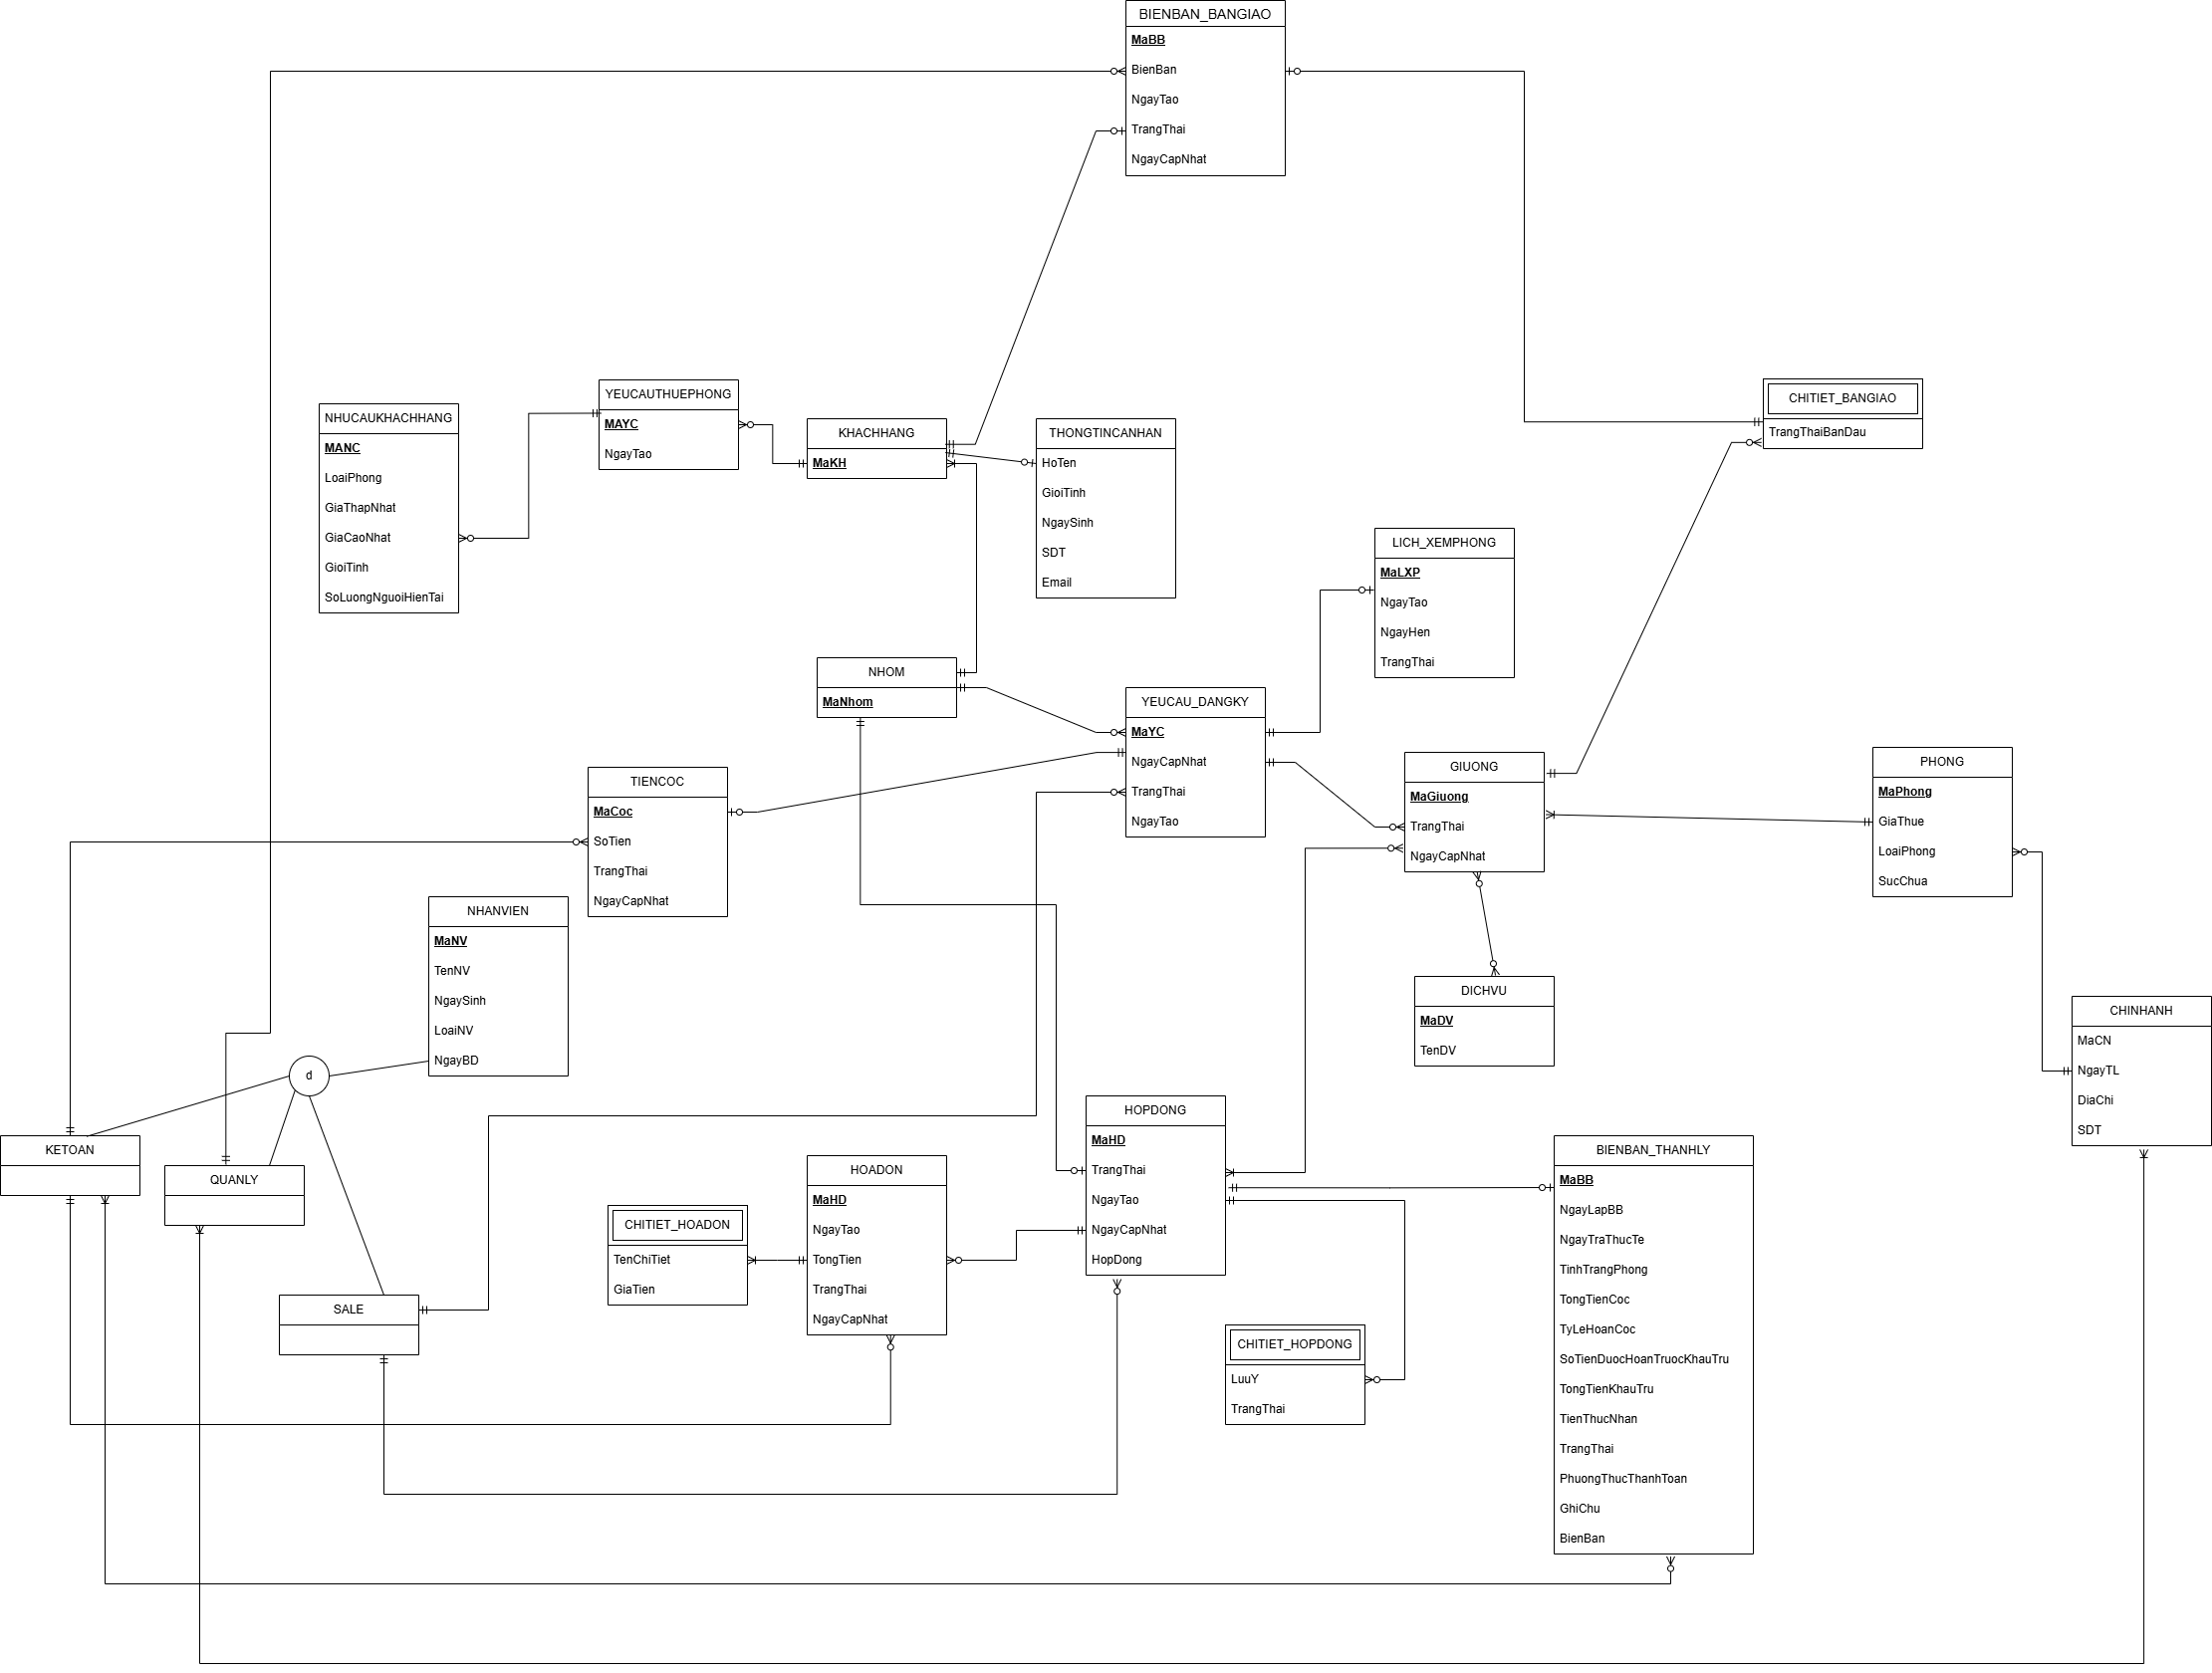
\includegraphics[width=0.98\textwidth]{images/ERD.drawio(1).png}
    \caption{Mô hình ERD của hệ thống HomeStay Dorm}
\end{figure}
